\documentclass[twoside]{book}

% Packages required by doxygen
\usepackage{fixltx2e}
\usepackage{calc}
\usepackage{doxygen}
\usepackage{graphicx}
\usepackage[utf8]{inputenc}
\usepackage{makeidx}
\usepackage{multicol}
\usepackage{multirow}
\PassOptionsToPackage{warn}{textcomp}
\usepackage{textcomp}
\usepackage[nointegrals]{wasysym}
\usepackage[table]{xcolor}

% Font selection
\usepackage[T1]{fontenc}
\usepackage{mathptmx}
\usepackage[scaled=.90]{helvet}
\usepackage{courier}
\usepackage{amssymb}
\usepackage{sectsty}
\renewcommand{\familydefault}{\sfdefault}
\allsectionsfont{%
  \fontseries{bc}\selectfont%
  \color{darkgray}%
}
\renewcommand{\DoxyLabelFont}{%
  \fontseries{bc}\selectfont%
  \color{darkgray}%
}
\newcommand{\+}{\discretionary{\mbox{\scriptsize$\hookleftarrow$}}{}{}}

% Page & text layout
\usepackage{geometry}
\geometry{%
  a4paper,%
  top=2.5cm,%
  bottom=2.5cm,%
  left=2.5cm,%
  right=2.5cm%
}
\tolerance=750
\hfuzz=15pt
\hbadness=750
\setlength{\emergencystretch}{15pt}
\setlength{\parindent}{0cm}
\setlength{\parskip}{0.2cm}
\makeatletter
\renewcommand{\paragraph}{%
  \@startsection{paragraph}{4}{0ex}{-1.0ex}{1.0ex}{%
    \normalfont\normalsize\bfseries\SS@parafont%
  }%
}
\renewcommand{\subparagraph}{%
  \@startsection{subparagraph}{5}{0ex}{-1.0ex}{1.0ex}{%
    \normalfont\normalsize\bfseries\SS@subparafont%
  }%
}
\makeatother

% Headers & footers
\usepackage{fancyhdr}
\pagestyle{fancyplain}
\fancyhead[LE]{\fancyplain{}{\bfseries\thepage}}
\fancyhead[CE]{\fancyplain{}{}}
\fancyhead[RE]{\fancyplain{}{\bfseries\leftmark}}
\fancyhead[LO]{\fancyplain{}{\bfseries\rightmark}}
\fancyhead[CO]{\fancyplain{}{}}
\fancyhead[RO]{\fancyplain{}{\bfseries\thepage}}
\fancyfoot[LE]{\fancyplain{}{}}
\fancyfoot[CE]{\fancyplain{}{}}
\fancyfoot[RE]{\fancyplain{}{\bfseries\scriptsize Generated on Tue Sep 30 2014 14\+:14\+:19 for vw4tools by Doxygen }}
\fancyfoot[LO]{\fancyplain{}{\bfseries\scriptsize Generated on Tue Sep 30 2014 14\+:14\+:19 for vw4tools by Doxygen }}
\fancyfoot[CO]{\fancyplain{}{}}
\fancyfoot[RO]{\fancyplain{}{}}
\renewcommand{\footrulewidth}{0.4pt}
\renewcommand{\chaptermark}[1]{%
  \markboth{#1}{}%
}
\renewcommand{\sectionmark}[1]{%
  \markright{\thesection\ #1}%
}

% Indices & bibliography
\usepackage{natbib}
\usepackage[titles]{tocloft}
\setcounter{tocdepth}{3}
\setcounter{secnumdepth}{5}
\makeindex

% Custom commands
\newcommand{\clearemptydoublepage}{%
  \newpage{\pagestyle{empty}\cleardoublepage}%
}


%===== C O N T E N T S =====

\begin{document}

% Titlepage & ToC
\pagenumbering{roman}
\begin{titlepage}
\vspace*{7cm}
\begin{center}%
{\Large vw4tools \\[1ex]\large 1.\+0-\/6 }\\
\vspace*{1cm}
{\large Generated by Doxygen 1.8.7}\\
\vspace*{0.5cm}
{\small Tue Sep 30 2014 14:14:19}\\
\end{center}
\end{titlepage}
\clearemptydoublepage
\tableofcontents
\clearemptydoublepage
\pagenumbering{arabic}

%--- Begin generated contents ---
\chapter{Java\+Doc A\+P\+I Markup for vw4tools}
\label{index}\section*{vw4tools }

Tools and utilities for Virtual\-Wisdom4 
\chapter{R\+E\+A\+D\+M\+E}
\label{md_htdocs_README}
\input{md_htdocs_README}
\chapter{Scripting Options}
\label{scripts}
\input{scripts}
\chapter{J\+V\+M Options}
\label{jvmopt}

\begin{DoxyRefList}
\item[\label{jvmopt__jvmopt000001}%
Global \doxyref{Entity.\+\_\+compatibility\+Version}{p.}{classorg_1_1smallfoot_1_1vw4_1_1Entity_a2d966176f7b315760e172d3bc03f64a1} ()]{\bfseries compat.\+target} (values\+: X.\+Y.\+Z as a version. For example\+: 4.\+0.\+1, 4.\+1, 4, 4.\+2) can be used to tell the J\+S\+O\+N output to use specific features available on later versions of the Virtual\+Wisdom4 product. Initially controls whether fcport entities are created but may expand.  
\item[\label{jvmopt__jvmopt000002}%
Global \doxyref{Virtual\+Wisdom4\+Client\+Tool.set\+Target}{p.}{classorg_1_1smallfoot_1_1vw4_1_1VirtualWisdom4ClientTool_adf6150f6553bb5d80b9c303817a94a9d} (String ver)]{\bfseries debug.\+show\+Compat\+Target} causes the compat.\+target to be displayed when (re)set 
\end{DoxyRefList}
\chapter{Todo List}
\label{todo}

\begin{DoxyRefList}
\item[\label{todo__todo000001}%
Global \doxyref{Virtual\+Wisdom4\+Client\+Tool.\+\_\+load}{p.}{classorg_1_1smallfoot_1_1vw4_1_1VirtualWisdom4ClientTool_ad9a051ba608e7fcb9adac39bc3946058} (String filename)]\+: evaluate\+: mapper.\+configure(Deserialization\+Config.\+Feature.\+F\+A\+I\+L\+\_\+\+O\+N\+\_\+\+U\+N\+K\+N\+O\+W\+N\+\_\+\+P\+R\+O\+P\+E\+R\+T\+I\+E\+S, false); 
\end{DoxyRefList}
\chapter{Commandline Options}
\label{cmdopt}

\begin{DoxyRefList}
\item[\label{cmdopt__cmdopt000001}%
Global \doxyref{Virtual\+Wisdom4\+Client\+Tool.main}{p.}{classorg_1_1smallfoot_1_1vw4_1_1VirtualWisdom4ClientTool_a75988cf84fc6ee7a2ebff36e363021aa} (String args\mbox{[}\mbox{]})]-\/\+H$\vert$--help Show a simple help screen as a reminder of options which are understood by the application 


\begin{DoxyCode}
java -jar vw4tools.jar --help 
\end{DoxyCode}


-\/\+V$\vert$--version Show the current release version for reference 


\begin{DoxyCode}
java -jar vw4tools.jar --version
 0.9-91 
\end{DoxyCode}


-\/n$\vert$--nicknameout=\{file\} Output nicknames from internal store 

-\/o$\vert$--output=\{file\} Output nicknames from internal store --nicknameout and --output are currently functionally identical; they both cause the internal nickname/entity base to be written out as J\+S\+O\+N with the exception of a few \char`\"{}magic\char`\"{} filenames\+:

1. {\bfseries schema.\+json} will cause the current schema to be written 

2. {\bfseries orderedtuples.\+csv} will cause an Ordered\+Tuples.\+csv file to be written, suitable for post-\/processing via \doxyref{csv-\/to-\/json.\+awk}{p.}{csv-to-json_8awk} but allowing a user to more easily edit C\+S\+V for fine-\/tuning 

3. {\bfseries orphanentities.\+csv} will cause a C\+S\+V to be written listing all orphan entities. An \char`\"{}\+Orphan Entity\char`\"{} is an entity lacking a parent entity, such as an \char`\"{}\+H\+B\+A Port\char`\"{} without a \char`\"{}host\char`\"{} parent, or a \char`\"{}iomodule\char`\"{} without a parent \char`\"{}storagearray\char`\"{} entity.

All other filename patterns will result in a J\+S\+O\+N-\/formatted file

-\/\+N$\vert$--nickname=\{file/uri\} Import nicknames by parsing a text stream from various sources 


\begin{DoxyCode}
java -jar vw4tools.jar --nickname=switch44.zoneshow
      Parse results \textcolor{keywordflow}{for} AliShowZoneParser:
      Zones: 44
      Aliases: 112 (names with one or more WWPNs)
      Aliases: 136 (name/WWPN tuples) 
\end{DoxyCode}
 In this example, a zone file was parsed by the Ali\+Show\+Zone\+Parser resulting in 112 nicknames; due to duplicate nicknames, there are actually 136 unique W\+W\+P\+N/alias tuples, which means that (136-\/112) 24 of the W\+W\+P\+Ns have the same alias as other W\+W\+P\+Ns

-\/i$\vert$--input import an existing J\+S\+O\+N file for later editing 

-\/r$\vert$--read import an existing J\+S\+O\+N file for later editing 


\begin{DoxyCode}
java -jar vw4tools.jar --read working.json 
\end{DoxyCode}


-\/\+R$\vert$--remove Parse ncknames for removal from the internal nickname list 

-\/\+R$\vert$--removenicknames Parse ncknames for removal from the internal nickname list

-\/!$\vert$--report Summarize the current status of the internal nicknaes and pattern/collation coverage 


\begin{DoxyCode}
java -jar vw4tools.jar --nickname=switch44.zoneshow  --report
(vw4tools) parsed 0 zones, 2 aliases via Alias4Parser
vw4tools 0.9-91
    5 total entities
    4 leaf nodes
    2 orphans
50.00 % coverage 
\end{DoxyCode}
 

-\/\+P$\vert$--pattern= is used to provide an \char`\"{}aggregating pattern\char`\"{} to collect Orphan Entities into a container. An \char`\"{}\+Orphan Entity\char`\"{} is an entity which is not part of a larger device\+: an H\+B\+A not assigned to a host, or a F\+A not assigned to a storage array. Aggregating Patterns are evaluated immediately, so their order amidst other command options to import or remove entities is important. 
\end{DoxyRefList}
\chapter{Hierarchical Index}
\section{Class Hierarchy}
This inheritance list is sorted roughly, but not completely, alphabetically\-:\begin{DoxyCompactList}
\item \contentsline{section}{V\-W\-Import.\-Edit\-\_\-\-Type}{\pageref{enumorg_1_1smallfoot_1_1vw4_1_1VWImport_1_1Edit__Type}}{}
\item \contentsline{section}{V\-W\-Import.\-Entity}{\pageref{classorg_1_1smallfoot_1_1vw4_1_1VWImport_1_1Entity}}{}
\item \contentsline{section}{Entity}{\pageref{classorg_1_1smallfoot_1_1vw4_1_1Entity}}{}
\begin{DoxyCompactList}
\item \contentsline{section}{Entity\-F\-A}{\pageref{classorg_1_1smallfoot_1_1vw4_1_1EntityFA}}{}
\item \contentsline{section}{Entity\-H\-B\-A}{\pageref{classorg_1_1smallfoot_1_1vw4_1_1EntityHBA}}{}
\end{DoxyCompactList}
\item Exception\begin{DoxyCompactList}
\item \contentsline{section}{Entity.\-Improper\-Child\-Exception}{\pageref{classorg_1_1smallfoot_1_1vw4_1_1Entity_1_1ImproperChildException}}{}
\end{DoxyCompactList}
\item \contentsline{section}{V\-W\-Import.\-I\-T\-L\-Pattern}{\pageref{classorg_1_1smallfoot_1_1vw4_1_1VWImport_1_1ITLPattern}}{}
\item \contentsline{section}{V\-W\-Import.\-Leaf\-Pattern}{\pageref{classorg_1_1smallfoot_1_1vw4_1_1VWImport_1_1LeafPattern}}{}
\item \contentsline{section}{Virtual\-Wisdom4\-Client\-Tool}{\pageref{classorg_1_1smallfoot_1_1vw4_1_1VirtualWisdom4ClientTool}}{}
\item \contentsline{section}{V\-W\-Import}{\pageref{classorg_1_1smallfoot_1_1vw4_1_1VWImport}}{}
\end{DoxyCompactList}

\chapter{Data Structure Index}
\section{Data Structures}
Here are the data structures with brief descriptions\-:\begin{DoxyCompactList}
\item\contentsline{section}{{\bf Virtual\-Wisdom4\-Client\-Tool} \\*X\-Path\-Tool is a relatively uncomplicated wrapper for an X\-Path action\-: it doesn't know what you're doing, and doesn't assume you'll do things in a specific order, but tries to stop you from making really silly errors like saving or searching an unloaded file }{\pageref{classorg_1_1smallfoot_1_1vw4_1_1VirtualWisdom4ClientTool}}{}
\end{DoxyCompactList}

\chapter{File Index}
\section{File List}
Here is a list of all documented files with brief descriptions\+:\begin{DoxyCompactList}
\item\contentsline{section}{java/{\bf Entity.\+java} }{\pageref{Entity_8java}}{}
\item\contentsline{section}{java/{\bf Entity\+Array.\+java} }{\pageref{EntityArray_8java}}{}
\item\contentsline{section}{java/{\bf Entity\+F\+A.\+java} }{\pageref{EntityFA_8java}}{}
\item\contentsline{section}{java/{\bf Entity\+H\+B\+A.\+java} }{\pageref{EntityHBA_8java}}{}
\item\contentsline{section}{java/{\bf Entity\+Host.\+java} }{\pageref{EntityHost_8java}}{}
\item\contentsline{section}{java/{\bf Virtual\+Wisdom4\+Client\+Tool.\+java} }{\pageref{VirtualWisdom4ClientTool_8java}}{}
\item\contentsline{section}{java/{\bf V\+W\+Import.\+java} }{\pageref{VWImport_8java}}{}
\item\contentsline{section}{scripts/{\bf csv-\/to-\/json.\+awk} }{\pageref{csv-to-json_8awk}}{}
\end{DoxyCompactList}

\chapter{Data Structure Documentation}
\section{Entity Class Reference}
\label{classorg_1_1smallfoot_1_1vw4_1_1Entity}\index{Entity@{Entity}}


An \doxyref{Entity}{p.}{classorg_1_1smallfoot_1_1vw4_1_1Entity} is the core mutable object used in the J\-S\-O\-N import for V\-W4.  




Collaboration diagram for Entity\-:\nopagebreak
\begin{figure}[H]
\begin{center}
\leavevmode
\includegraphics[width=176pt]{classorg_1_1smallfoot_1_1vw4_1_1Entity__coll__graph}
\end{center}
\end{figure}
\subsection*{Data Structures}
\begin{DoxyCompactItemize}
\item 
class {\bf Improper\-Child\-Exception}
\begin{DoxyCompactList}\small\item\em Descendents of \doxyref{Entity}{p.}{classorg_1_1smallfoot_1_1vw4_1_1Entity} should know whether a given entity can be one of their child elements. \end{DoxyCompactList}\end{DoxyCompactItemize}
\subsection*{Public Member Functions}
\begin{DoxyCompactItemize}
\item 
{\bf Entity} (String {\bf name})\label{classorg_1_1smallfoot_1_1vw4_1_1Entity_afc6a43ee8007bcc023a7ebd2bf5ee1ed}

\begin{DoxyCompactList}\small\item\em Class Constructor with no initial child. \end{DoxyCompactList}\item 
{\bf Entity} (String {\bf name}, {\bf Entity} e)  throws Improper\-Child\-Exception     \label{classorg_1_1smallfoot_1_1vw4_1_1Entity_a1afb3a328033f8f6bf136d8380e712b9}

\begin{DoxyCompactList}\small\item\em Class Constructor with an initial child to absorb. \end{DoxyCompactList}\end{DoxyCompactItemize}
\subsection*{Protected Member Functions}
\begin{DoxyCompactItemize}
\item 
abstract boolean {\bf can\-Be\-Child} ({\bf Entity} e)
\begin{DoxyCompactList}\small\item\em whether a given entity can be this entity's child \end{DoxyCompactList}\item 
Vector$<$ {\bf Entity} $>$ {\bf children} ()\label{classorg_1_1smallfoot_1_1vw4_1_1Entity_a63ef33ad49b88027164e49d1916f409c}

\begin{DoxyCompactList}\small\item\em local access to local singleton .children \end{DoxyCompactList}\end{DoxyCompactItemize}
\subsection*{Protected Attributes}
\begin{DoxyCompactItemize}
\item 
Vector$<$ {\bf Entity} $>$ {\bf children} = null\label{classorg_1_1smallfoot_1_1vw4_1_1Entity_ad315cf5c2790d5a5c8c5169c26647e84}

\begin{DoxyCompactList}\small\item\em local singleton late-\/instantiated as needed by \doxyref{children()}{p.}{classorg_1_1smallfoot_1_1vw4_1_1Entity_a63ef33ad49b88027164e49d1916f409c} \end{DoxyCompactList}\item 
String {\bf name}\label{classorg_1_1smallfoot_1_1vw4_1_1Entity_a9a2326f35466e54c36c070829245c557}

\begin{DoxyCompactList}\small\item\em the unique name of the entity \end{DoxyCompactList}\end{DoxyCompactItemize}


\subsection{Detailed Description}
An \doxyref{Entity}{p.}{classorg_1_1smallfoot_1_1vw4_1_1Entity} is the core mutable object used in the J\-S\-O\-N import for V\-W4. 

I'm not so sure how it'll unfold yet, but I intend to treat all hosts and hbas and storagecontrollers and iomodules as similar objects\-: things that can have children things. In the short term, be very careful\-: there is an \doxyref{Entity}{p.}{classorg_1_1smallfoot_1_1vw4_1_1Entity}, and a \doxyref{V\-W\-Import\-::\-Entity}{p.}{classorg_1_1smallfoot_1_1vw4_1_1VWImport_1_1Entity} 

Definition at line 44 of file Entity.\-java.



\subsection{Member Function Documentation}
\index{org\-::smallfoot\-::vw4\-::\-Entity@{org\-::smallfoot\-::vw4\-::\-Entity}!can\-Be\-Child@{can\-Be\-Child}}
\index{can\-Be\-Child@{can\-Be\-Child}!org::smallfoot::vw4::Entity@{org\-::smallfoot\-::vw4\-::\-Entity}}
\subsubsection[{can\-Be\-Child}]{\setlength{\rightskip}{0pt plus 5cm}abstract boolean can\-Be\-Child (
\begin{DoxyParamCaption}
\item[{{\bf Entity}}]{e}
\end{DoxyParamCaption}
)\hspace{0.3cm}{\ttfamily [abstract]}, {\ttfamily [protected]}}\label{classorg_1_1smallfoot_1_1vw4_1_1Entity_a0a8c67a491e7100ba94f3035bbe62822}


whether a given entity can be this entity's child 

\begin{DoxyReturn}{Returns}
true if accepted, false if refused 
\end{DoxyReturn}

\begin{DoxyParams}{Parameters}
{\em e} & entity to check for possible descendent-\/hood \\
\hline
\end{DoxyParams}


Referenced by Entity.\-Entity().



The documentation for this class was generated from the following file\-:\begin{DoxyCompactItemize}
\item 
java/{\bf Entity.\-java}\end{DoxyCompactItemize}

\section{Entity\+Array Class Reference}
\label{classorg_1_1smallfoot_1_1vw4_1_1EntityArray}\index{Entity\+Array@{Entity\+Array}}


An \doxyref{Entity\+Array}{p.}{classorg_1_1smallfoot_1_1vw4_1_1EntityArray} is the representation of an Array entity in the J\+S\+O\+N import for V\+W4.  




Inheritance diagram for Entity\+Array\+:\nopagebreak
\begin{figure}[H]
\begin{center}
\leavevmode
\includegraphics[width=108pt]{classorg_1_1smallfoot_1_1vw4_1_1EntityArray__inherit__graph}
\end{center}
\end{figure}


Collaboration diagram for Entity\+Array\+:\nopagebreak
\begin{figure}[H]
\begin{center}
\leavevmode
\includegraphics[width=350pt]{classorg_1_1smallfoot_1_1vw4_1_1EntityArray__coll__graph}
\end{center}
\end{figure}
\subsection*{Public Member Functions}
\begin{DoxyCompactItemize}
\item 
{\bf Entity\+Array} (String {\bf name}, {\bf Entity} e)  throws Improper\+Child\+Exception     \label{classorg_1_1smallfoot_1_1vw4_1_1EntityArray_a82720c65ff67c93dc762f047d8916488}

\begin{DoxyCompactList}\small\item\em Basic Class Constructor. \end{DoxyCompactList}\item 
{\bf Entity} {\bf new\+Parent} (String {\bf name})\label{classorg_1_1smallfoot_1_1vw4_1_1EntityArray_ae3cca685b4cef300a70d257f519a96e4}

\begin{DoxyCompactList}\small\item\em create a new \doxyref{Entity}{p.}{classorg_1_1smallfoot_1_1vw4_1_1Entity} of the correct class to be a parent of this one \end{DoxyCompactList}\end{DoxyCompactItemize}
\subsection*{Protected Member Functions}
\begin{DoxyCompactItemize}
\item 
boolean {\bf can\+Be\+Child} ({\bf Entity} e)
\begin{DoxyCompactList}\small\item\em whether a given entity can be this entity's child \end{DoxyCompactList}\item 
org.\+smallfoot.\+vw4.\+V\+W\+Import.\+Entity {\bf vwentity} (String tag)
\begin{DoxyCompactList}\small\item\em create a streamable J\+S\+O\+N entity from this one \end{DoxyCompactList}\end{DoxyCompactItemize}
\subsection*{Additional Inherited Members}


\subsection{Detailed Description}
An \doxyref{Entity\+Array}{p.}{classorg_1_1smallfoot_1_1vw4_1_1EntityArray} is the representation of an Array entity in the J\+S\+O\+N import for V\+W4. 

Be very careful\+: there is an \doxyref{Entity}{p.}{classorg_1_1smallfoot_1_1vw4_1_1Entity}, and a V\+W\+Import\+::\+Entity 

Definition at line 44 of file Entity\+Array.\+java.



\subsection{Member Function Documentation}
\index{org\+::smallfoot\+::vw4\+::\+Entity\+Array@{org\+::smallfoot\+::vw4\+::\+Entity\+Array}!can\+Be\+Child@{can\+Be\+Child}}
\index{can\+Be\+Child@{can\+Be\+Child}!org\+::smallfoot\+::vw4\+::\+Entity\+Array@{org\+::smallfoot\+::vw4\+::\+Entity\+Array}}
\subsubsection[{can\+Be\+Child}]{\setlength{\rightskip}{0pt plus 5cm}boolean can\+Be\+Child (
\begin{DoxyParamCaption}
\item[{{\bf Entity}}]{e}
\end{DoxyParamCaption}
)\hspace{0.3cm}{\ttfamily [inline]}, {\ttfamily [protected]}}\label{classorg_1_1smallfoot_1_1vw4_1_1EntityArray_a5a51654ce8be38d5f06faa182cb70e61}


whether a given entity can be this entity's child 

\begin{DoxyReturn}{Returns}
true if accepted, false if refused 
\end{DoxyReturn}

\begin{DoxyParams}{Parameters}
{\em e} & entity to check for possible descendent-\/hood \\
\hline
\end{DoxyParams}


Definition at line 55 of file Entity\+Array.\+java.

\index{org\+::smallfoot\+::vw4\+::\+Entity\+Array@{org\+::smallfoot\+::vw4\+::\+Entity\+Array}!vwentity@{vwentity}}
\index{vwentity@{vwentity}!org\+::smallfoot\+::vw4\+::\+Entity\+Array@{org\+::smallfoot\+::vw4\+::\+Entity\+Array}}
\subsubsection[{vwentity}]{\setlength{\rightskip}{0pt plus 5cm}org.\+smallfoot.\+vw4.\+V\+W\+Import.\+Entity vwentity (
\begin{DoxyParamCaption}
\item[{String}]{tag}
\end{DoxyParamCaption}
)\hspace{0.3cm}{\ttfamily [inline]}, {\ttfamily [protected]}}\label{classorg_1_1smallfoot_1_1vw4_1_1EntityArray_a1d6bf85ddf0a9382cfa4f82dd3063473}


create a streamable J\+S\+O\+N entity from this one 

\begin{DoxyReturn}{Returns}
a org.\+smallfoot.\+vw4.\+V\+W\+Import.\+Entity representation of this instance 
\end{DoxyReturn}

\begin{DoxyParams}{Parameters}
{\em tag} & default tag to apply \\
\hline
\end{DoxyParams}


Definition at line 61 of file Entity\+Array.\+java.



References Entity.\+children(), Entity.\+description(), and Entity.\+name().



Here is the call graph for this function\+:\nopagebreak
\begin{figure}[H]
\begin{center}
\leavevmode
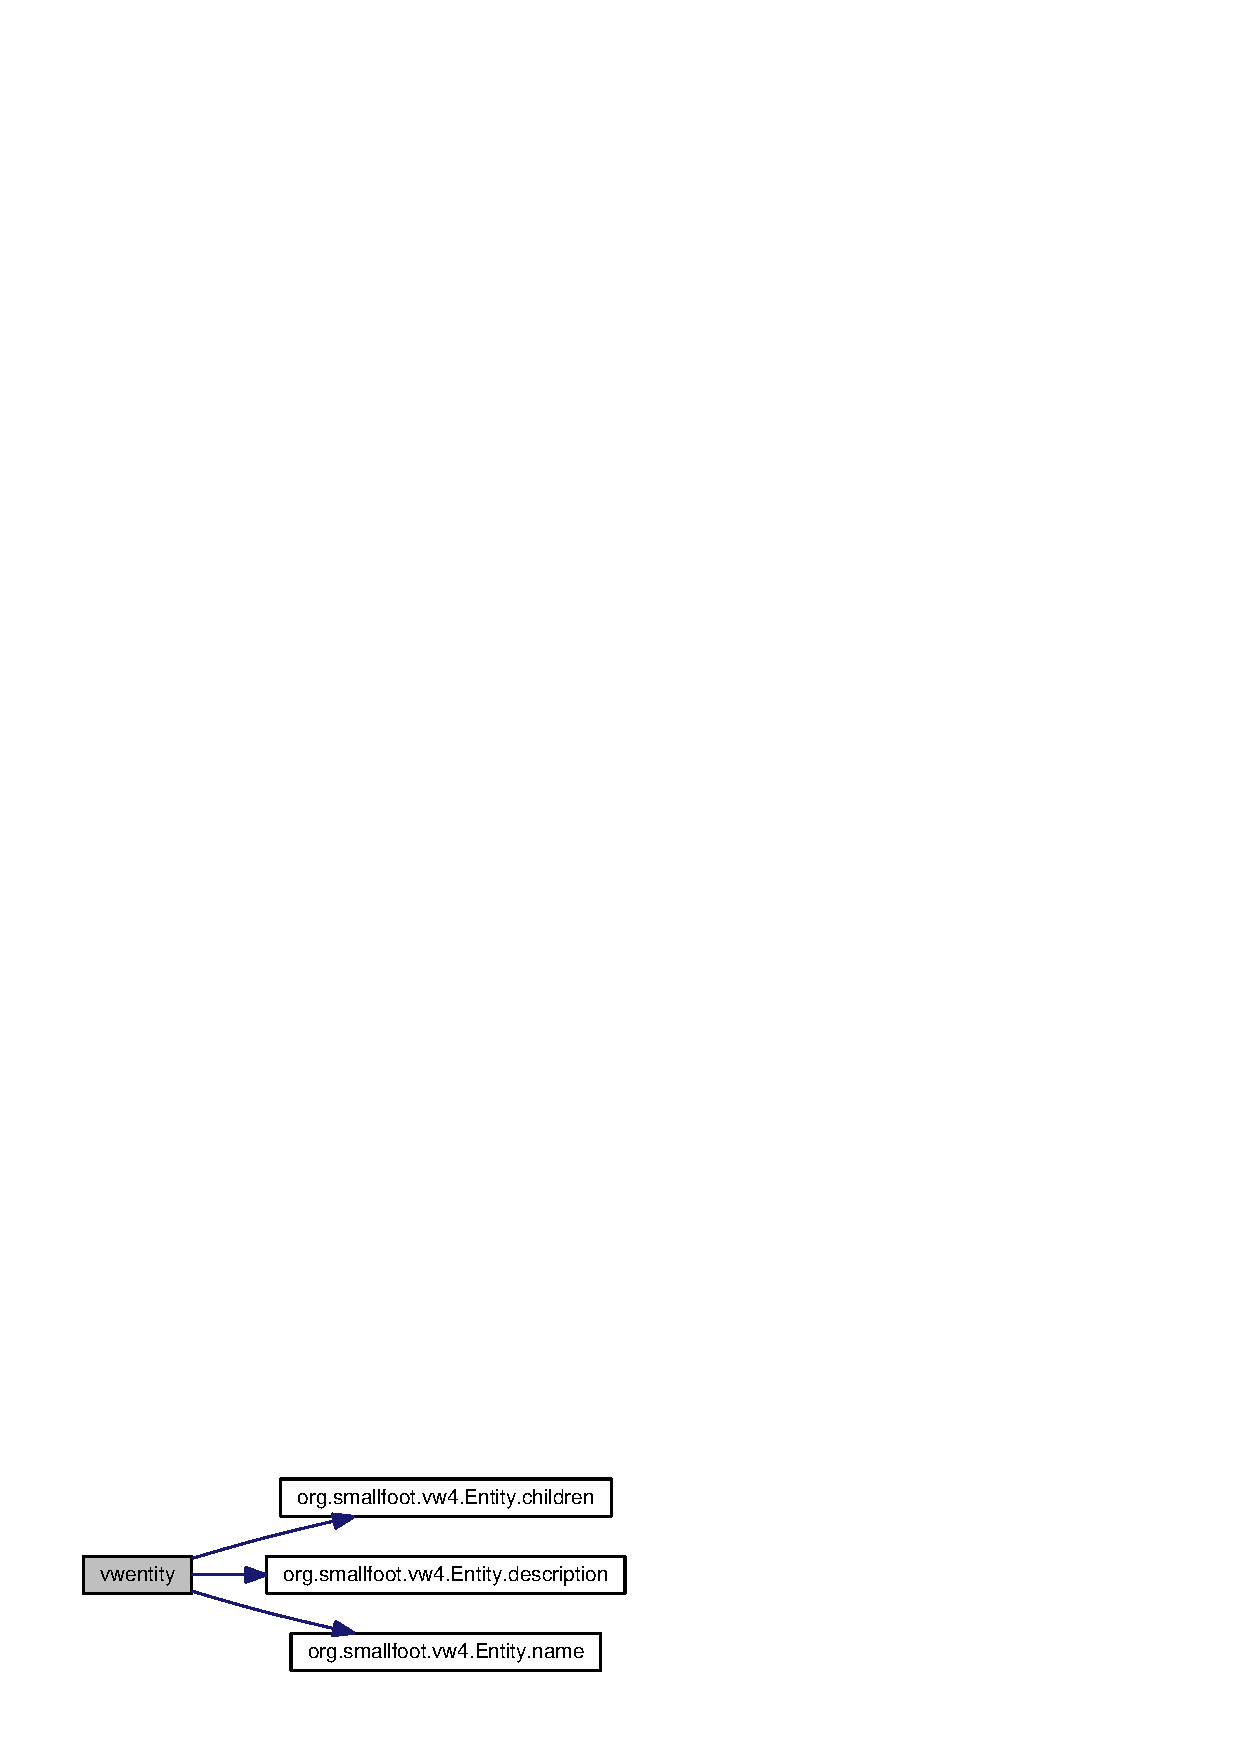
\includegraphics[width=304pt]{classorg_1_1smallfoot_1_1vw4_1_1EntityArray_a1d6bf85ddf0a9382cfa4f82dd3063473_cgraph}
\end{center}
\end{figure}




The documentation for this class was generated from the following file\+:\begin{DoxyCompactItemize}
\item 
java/{\bf Entity\+Array.\+java}\end{DoxyCompactItemize}

\section{Entity\-F\-A Class Reference}
\label{classorg_1_1smallfoot_1_1vw4_1_1EntityFA}\index{Entity\-F\-A@{Entity\-F\-A}}


An \doxyref{Entity\-F\-A}{p.}{classorg_1_1smallfoot_1_1vw4_1_1EntityFA} is the representation of an Storage F\-A entity in the J\-S\-O\-N import for V\-W4.  




Inheritance diagram for Entity\-F\-A\-:\nopagebreak
\begin{figure}[H]
\begin{center}
\leavevmode
\includegraphics[width=96pt]{classorg_1_1smallfoot_1_1vw4_1_1EntityFA__inherit__graph}
\end{center}
\end{figure}


Collaboration diagram for Entity\-F\-A\-:\nopagebreak
\begin{figure}[H]
\begin{center}
\leavevmode
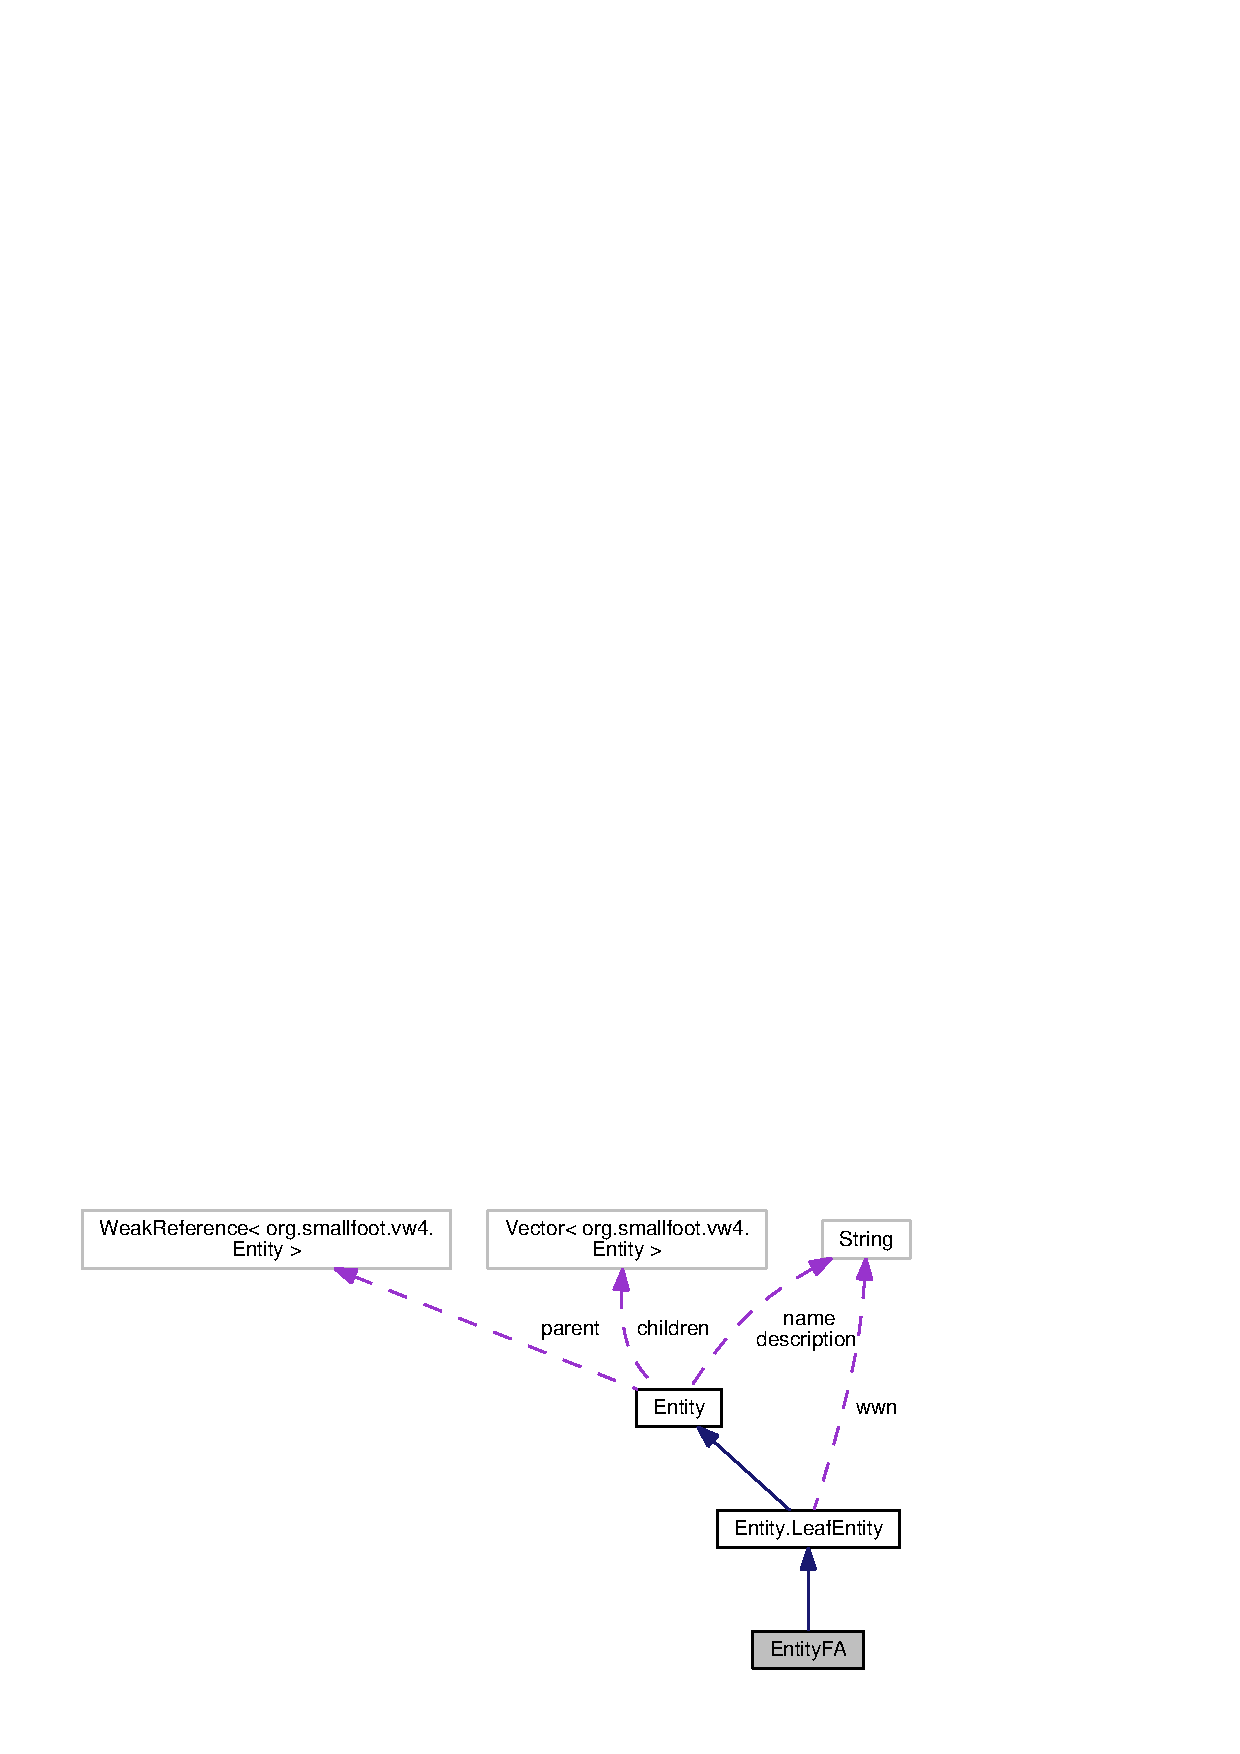
\includegraphics[width=350pt]{classorg_1_1smallfoot_1_1vw4_1_1EntityFA__coll__graph}
\end{center}
\end{figure}
\subsection*{Public Member Functions}
\begin{DoxyCompactItemize}
\item 
{\bf Entity\-F\-A} (String {\bf name}, String {\bf wwn})\label{classorg_1_1smallfoot_1_1vw4_1_1EntityFA_aee1f13fcac25df5320b16ca060ad99dd}

\begin{DoxyCompactList}\small\item\em Class Constructor with no initial child. \end{DoxyCompactList}\item 
String {\bf wwn} ()\label{classorg_1_1smallfoot_1_1vw4_1_1EntityFA_aa0f20764b2a9bea375e9507de63cb42b}

\begin{DoxyCompactList}\small\item\em getter \end{DoxyCompactList}\end{DoxyCompactItemize}
\subsection*{Protected Member Functions}
\begin{DoxyCompactItemize}
\item 
boolean {\bf can\-Be\-Child} ({\bf Entity} e)\label{classorg_1_1smallfoot_1_1vw4_1_1EntityFA_a5a51654ce8be38d5f06faa182cb70e61}

\begin{DoxyCompactList}\small\item\em this entity has no children so this method will always be false \end{DoxyCompactList}\item 
{\bf org.\-smallfoot.\-vw4.\-V\-W\-Import.\-Entity} {\bf vwentity} ()
\begin{DoxyCompactList}\small\item\em create a streamable J\-S\-O\-N entity from this one \end{DoxyCompactList}\end{DoxyCompactItemize}
\subsection*{Protected Attributes}
\begin{DoxyCompactItemize}
\item 
String {\bf wwn}\label{classorg_1_1smallfoot_1_1vw4_1_1EntityFA_ab07f595ad2e4da7c53cd29f435f5bb3c}

\begin{DoxyCompactList}\small\item\em the unique W\-W\-P\-N of the hba \end{DoxyCompactList}\end{DoxyCompactItemize}


\subsection{Detailed Description}
An \doxyref{Entity\-F\-A}{p.}{classorg_1_1smallfoot_1_1vw4_1_1EntityFA} is the representation of an Storage F\-A entity in the J\-S\-O\-N import for V\-W4. 

Be very careful\-: there is an \doxyref{Entity}{p.}{classorg_1_1smallfoot_1_1vw4_1_1Entity}, and a \doxyref{V\-W\-Import\-::\-Entity}{p.}{classorg_1_1smallfoot_1_1vw4_1_1VWImport_1_1Entity} 

Definition at line 44 of file Entity\-F\-A.\-java.



\subsection{Member Function Documentation}
\index{org\-::smallfoot\-::vw4\-::\-Entity\-F\-A@{org\-::smallfoot\-::vw4\-::\-Entity\-F\-A}!vwentity@{vwentity}}
\index{vwentity@{vwentity}!org::smallfoot::vw4::EntityFA@{org\-::smallfoot\-::vw4\-::\-Entity\-F\-A}}
\subsubsection[{vwentity}]{\setlength{\rightskip}{0pt plus 5cm}{\bf org.\-smallfoot.\-vw4.\-V\-W\-Import.\-Entity} vwentity (
\begin{DoxyParamCaption}
{}
\end{DoxyParamCaption}
)\hspace{0.3cm}{\ttfamily [inline]}, {\ttfamily [protected]}}\label{classorg_1_1smallfoot_1_1vw4_1_1EntityFA_abbe45f145f6cb53a7e9b67b576c42a9e}


create a streamable J\-S\-O\-N entity from this one 

\begin{DoxyReturn}{Returns}
a \doxyref{org.\-smallfoot.\-vw4.\-V\-W\-Import.\-Entity}{p.}{classorg_1_1smallfoot_1_1vw4_1_1VWImport_1_1Entity} representation of this instance 
\end{DoxyReturn}


Definition at line 62 of file Entity\-F\-A.\-java.



References Entity.\-description(), Entity.\-name(), and Entity\-F\-A.\-wwn().



Here is the call graph for this function\-:\nopagebreak
\begin{figure}[H]
\begin{center}
\leavevmode
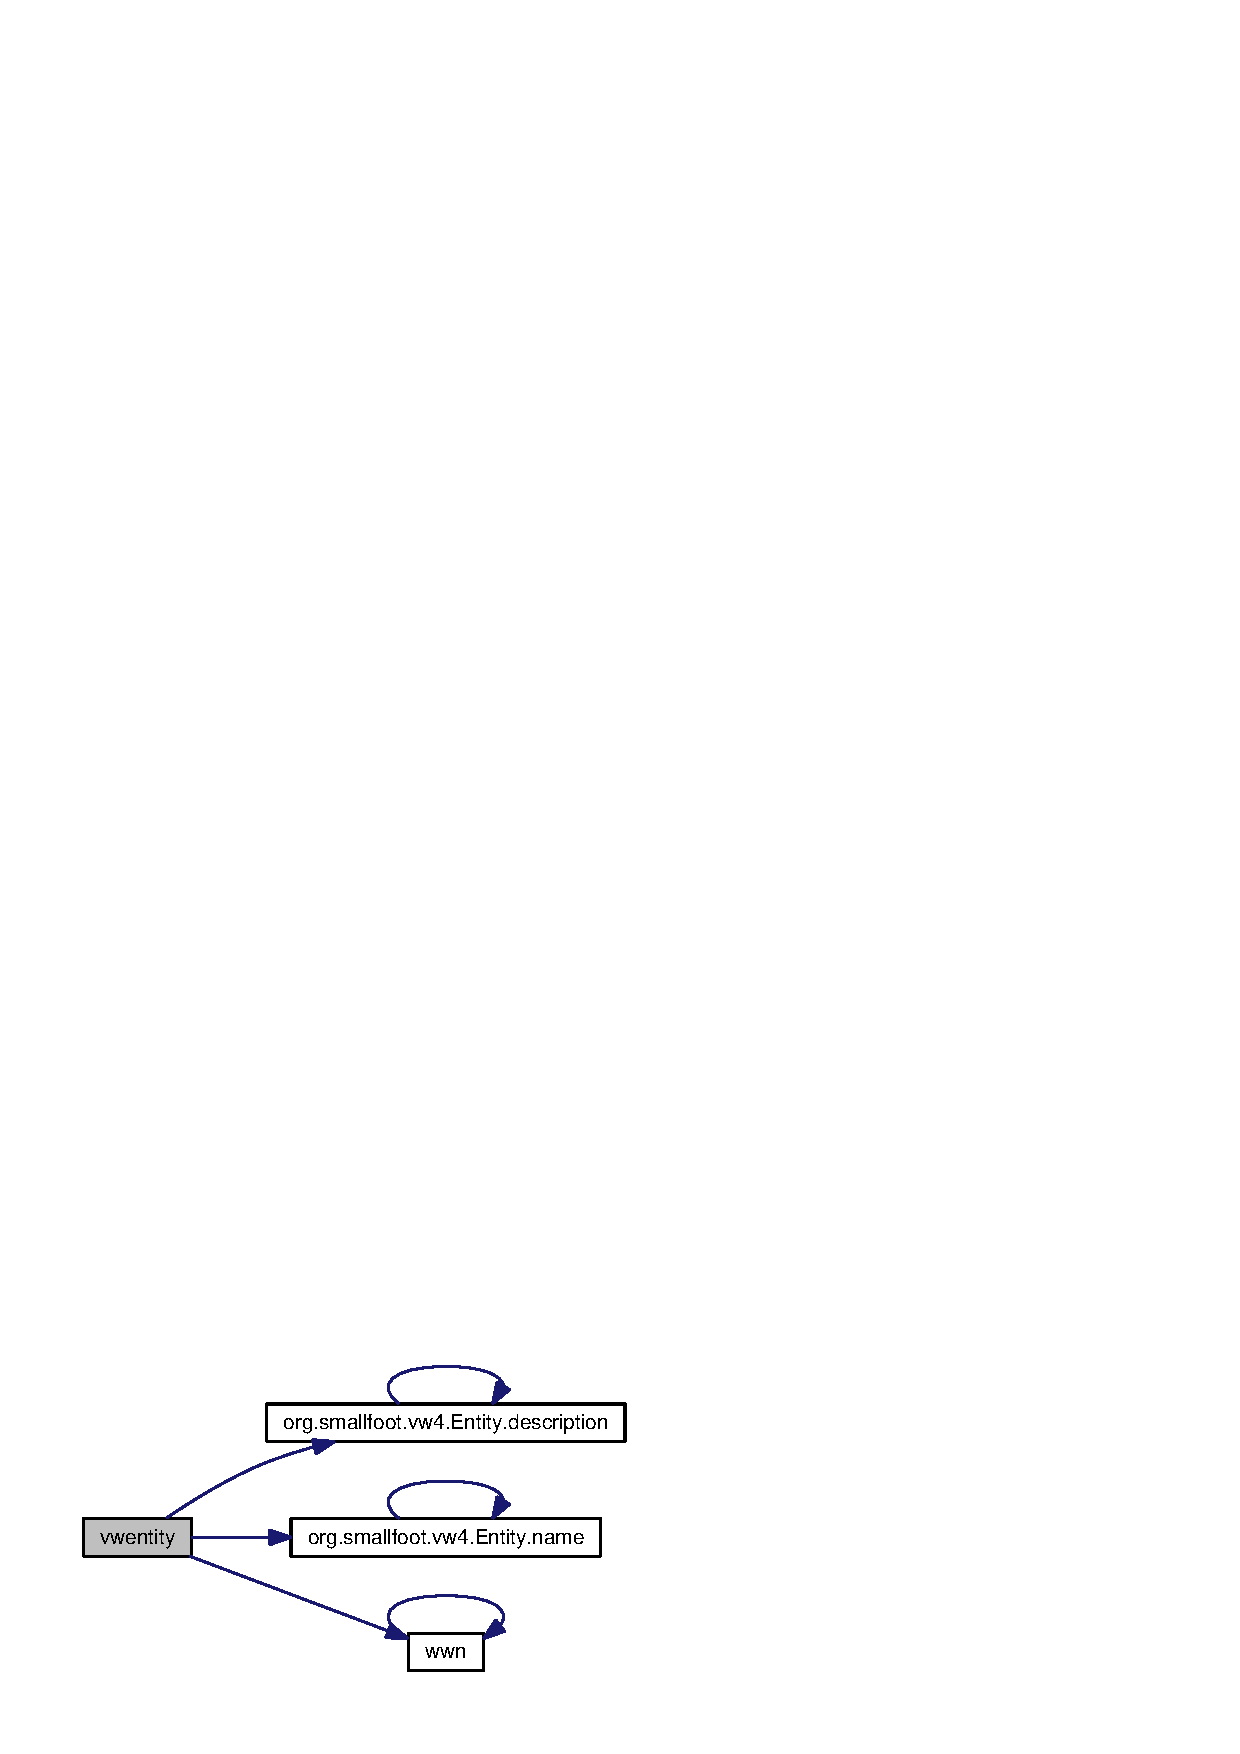
\includegraphics[width=304pt]{classorg_1_1smallfoot_1_1vw4_1_1EntityFA_abbe45f145f6cb53a7e9b67b576c42a9e_cgraph}
\end{center}
\end{figure}




The documentation for this class was generated from the following file\-:\begin{DoxyCompactItemize}
\item 
java/{\bf Entity\-F\-A.\-java}\end{DoxyCompactItemize}

\section{Entity\+H\+B\+A Class Reference}
\label{classorg_1_1smallfoot_1_1vw4_1_1EntityHBA}\index{Entity\+H\+B\+A@{Entity\+H\+B\+A}}


An \doxyref{Entity\+H\+B\+A}{p.}{classorg_1_1smallfoot_1_1vw4_1_1EntityHBA} is the representation of an H\+B\+A entity in the J\+S\+O\+N import for V\+W4.  




Inheritance diagram for Entity\+H\+B\+A\+:\nopagebreak
\begin{figure}[H]
\begin{center}
\leavevmode
\includegraphics[width=130pt]{classorg_1_1smallfoot_1_1vw4_1_1EntityHBA__inherit__graph}
\end{center}
\end{figure}


Collaboration diagram for Entity\+H\+B\+A\+:\nopagebreak
\begin{figure}[H]
\begin{center}
\leavevmode
\includegraphics[width=350pt]{classorg_1_1smallfoot_1_1vw4_1_1EntityHBA__coll__graph}
\end{center}
\end{figure}
\subsection*{Public Member Functions}
\begin{DoxyCompactItemize}
\item 
{\bf Entity\+H\+B\+A} (String {\bf name}, String {\bf wwn})\label{classorg_1_1smallfoot_1_1vw4_1_1EntityHBA_a5470c9c351f0ea8dd64d612e11c7214f}

\begin{DoxyCompactList}\small\item\em Basic Class Constructor. \end{DoxyCompactList}\item 
{\bf Entity} {\bf new\+Parent} (String {\bf name})\label{classorg_1_1smallfoot_1_1vw4_1_1EntityHBA_ae3cca685b4cef300a70d257f519a96e4}

\begin{DoxyCompactList}\small\item\em create a new \doxyref{Entity}{p.}{classorg_1_1smallfoot_1_1vw4_1_1Entity} of the correct class to be a parent of this one \end{DoxyCompactList}\end{DoxyCompactItemize}
\subsection*{Protected Member Functions}
\begin{DoxyCompactItemize}
\item 
org.\+smallfoot.\+vw4.\+V\+W\+Import.\+Entity {\bf vwentity} (String tag)
\begin{DoxyCompactList}\small\item\em create a streamable J\+S\+O\+N entity from this one \end{DoxyCompactList}\end{DoxyCompactItemize}
\subsection*{Additional Inherited Members}


\subsection{Detailed Description}
An \doxyref{Entity\+H\+B\+A}{p.}{classorg_1_1smallfoot_1_1vw4_1_1EntityHBA} is the representation of an H\+B\+A entity in the J\+S\+O\+N import for V\+W4. 

Be very careful\+: there is an \doxyref{Entity}{p.}{classorg_1_1smallfoot_1_1vw4_1_1Entity}, and a V\+W\+Import\+::\+Entity 

Definition at line 44 of file Entity\+H\+B\+A.\+java.



\subsection{Member Function Documentation}
\index{org\+::smallfoot\+::vw4\+::\+Entity\+H\+B\+A@{org\+::smallfoot\+::vw4\+::\+Entity\+H\+B\+A}!vwentity@{vwentity}}
\index{vwentity@{vwentity}!org\+::smallfoot\+::vw4\+::\+Entity\+H\+B\+A@{org\+::smallfoot\+::vw4\+::\+Entity\+H\+B\+A}}
\subsubsection[{vwentity}]{\setlength{\rightskip}{0pt plus 5cm}org.\+smallfoot.\+vw4.\+V\+W\+Import.\+Entity vwentity (
\begin{DoxyParamCaption}
\item[{String}]{tag}
\end{DoxyParamCaption}
)\hspace{0.3cm}{\ttfamily [inline]}, {\ttfamily [protected]}}\label{classorg_1_1smallfoot_1_1vw4_1_1EntityHBA_a1d6bf85ddf0a9382cfa4f82dd3063473}


create a streamable J\+S\+O\+N entity from this one 

\begin{DoxyReturn}{Returns}
a org.\+smallfoot.\+vw4.\+V\+W\+Import.\+Entity representation of this instance 
\end{DoxyReturn}

\begin{DoxyParams}{Parameters}
{\em tag} & default tag to apply \\
\hline
\end{DoxyParams}


Definition at line 55 of file Entity\+H\+B\+A.\+java.



References Entity.\+\_\+compatibility\+Version(), Entity.\+description(), Entity.\+name(), and Entity.\+Leaf\+Entity.\+wwn().



Here is the call graph for this function\+:\nopagebreak
\begin{figure}[H]
\begin{center}
\leavevmode
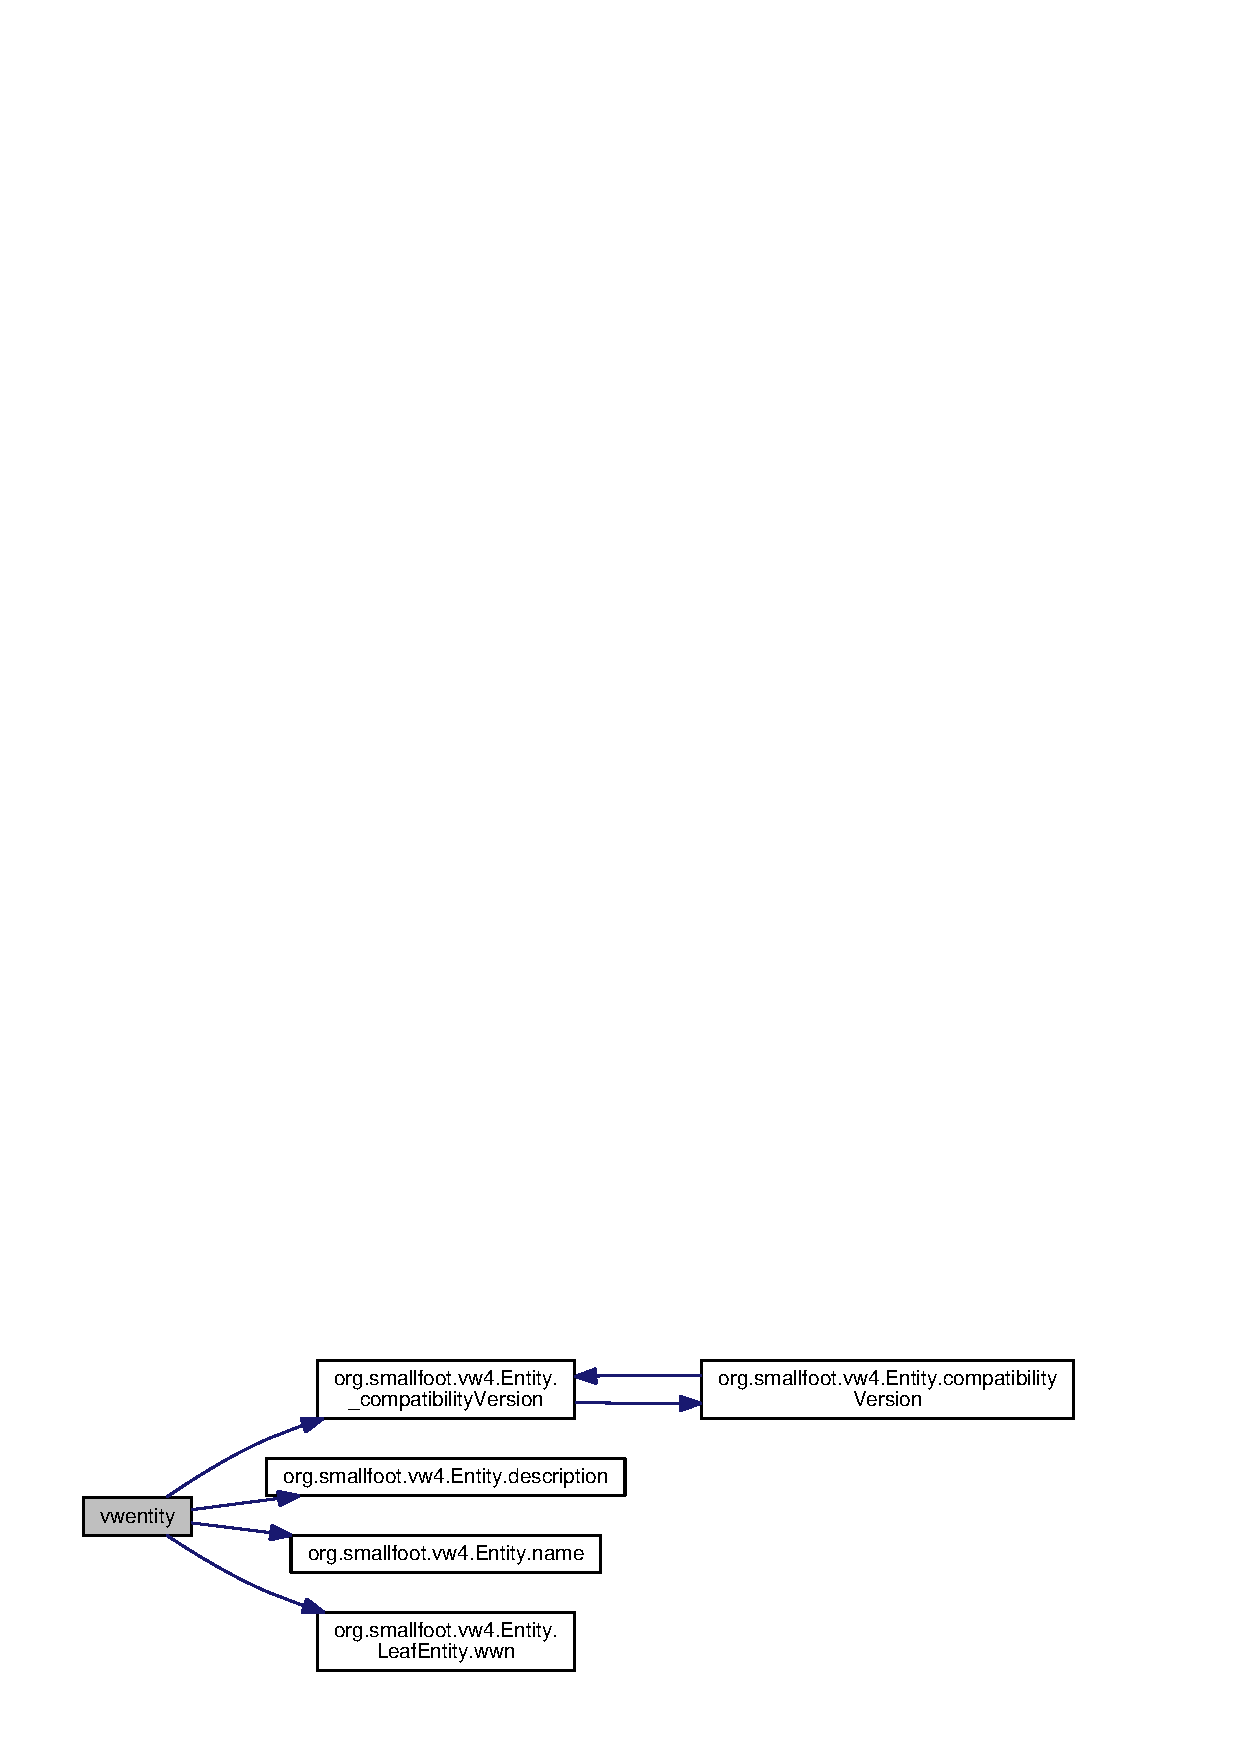
\includegraphics[width=350pt]{classorg_1_1smallfoot_1_1vw4_1_1EntityHBA_a1d6bf85ddf0a9382cfa4f82dd3063473_cgraph}
\end{center}
\end{figure}




The documentation for this class was generated from the following file\+:\begin{DoxyCompactItemize}
\item 
java/{\bf Entity\+H\+B\+A.\+java}\end{DoxyCompactItemize}

\section{Entity\+Host Class Reference}
\label{classorg_1_1smallfoot_1_1vw4_1_1EntityHost}\index{Entity\+Host@{Entity\+Host}}


An \doxyref{Entity\+Host}{p.}{classorg_1_1smallfoot_1_1vw4_1_1EntityHost} is the representation of an Host entity in the J\+S\+O\+N import for V\+W4.  




Inheritance diagram for Entity\+Host\+:\nopagebreak
\begin{figure}[H]
\begin{center}
\leavevmode
\includegraphics[width=104pt]{classorg_1_1smallfoot_1_1vw4_1_1EntityHost__inherit__graph}
\end{center}
\end{figure}


Collaboration diagram for Entity\+Host\+:\nopagebreak
\begin{figure}[H]
\begin{center}
\leavevmode
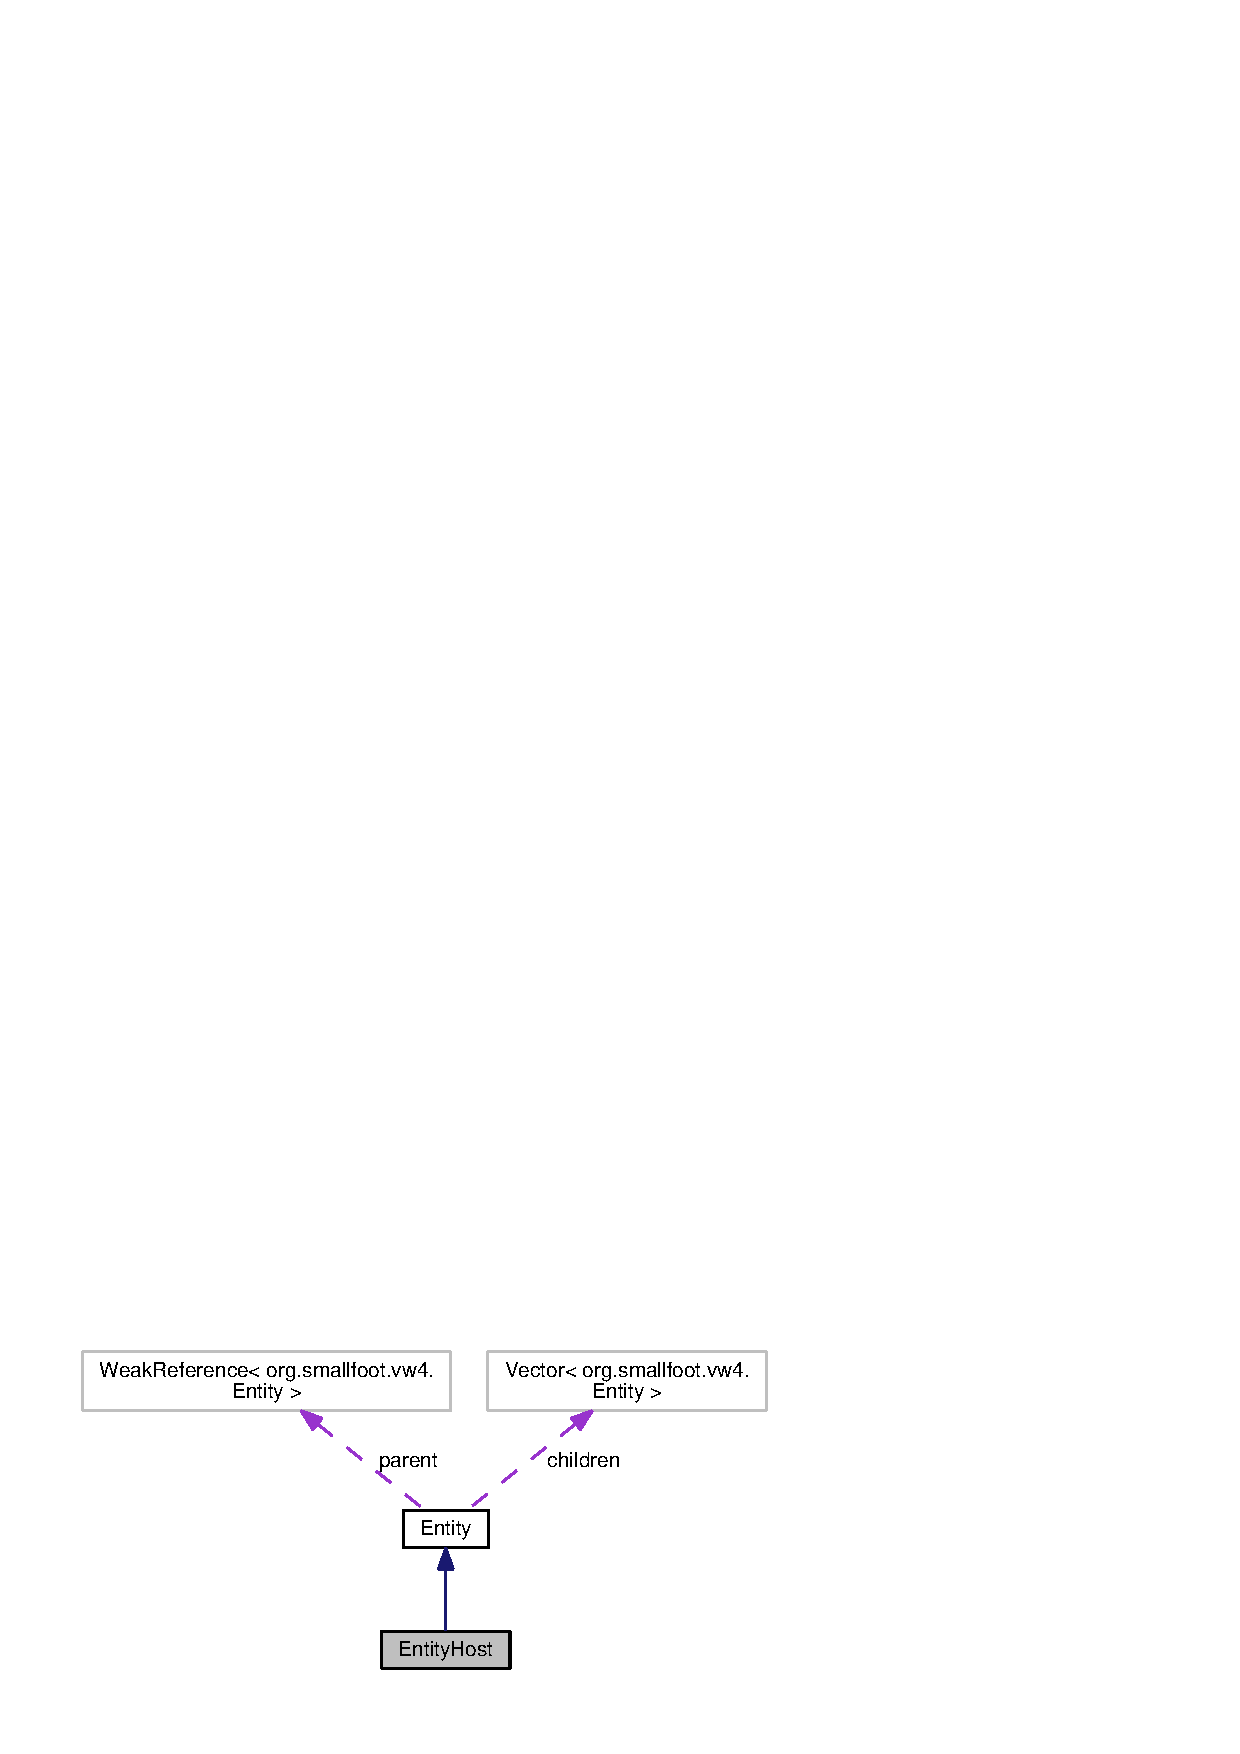
\includegraphics[width=350pt]{classorg_1_1smallfoot_1_1vw4_1_1EntityHost__coll__graph}
\end{center}
\end{figure}
\subsection*{Public Member Functions}
\begin{DoxyCompactItemize}
\item 
{\bf Entity\+Host} (String {\bf name}, {\bf Entity} e)  throws Improper\+Child\+Exception     \label{classorg_1_1smallfoot_1_1vw4_1_1EntityHost_a8c76d8db7cbedb53bd3469b0ec940962}

\begin{DoxyCompactList}\small\item\em Basic Class Constructor. \end{DoxyCompactList}\item 
{\bf Entity} {\bf new\+Parent} (String {\bf name})\label{classorg_1_1smallfoot_1_1vw4_1_1EntityHost_ae3cca685b4cef300a70d257f519a96e4}

\begin{DoxyCompactList}\small\item\em create a new \doxyref{Entity}{p.}{classorg_1_1smallfoot_1_1vw4_1_1Entity} of the correct class to be a parent of this one \end{DoxyCompactList}\end{DoxyCompactItemize}
\subsection*{Protected Member Functions}
\begin{DoxyCompactItemize}
\item 
boolean {\bf can\+Be\+Child} ({\bf Entity} e)
\begin{DoxyCompactList}\small\item\em whether a given entity can be this entity's child \end{DoxyCompactList}\item 
org.\+smallfoot.\+vw4.\+V\+W\+Import.\+Entity {\bf vwentity} (String tag)
\begin{DoxyCompactList}\small\item\em create a streamable J\+S\+O\+N entity from this one \end{DoxyCompactList}\end{DoxyCompactItemize}
\subsection*{Additional Inherited Members}


\subsection{Detailed Description}
An \doxyref{Entity\+Host}{p.}{classorg_1_1smallfoot_1_1vw4_1_1EntityHost} is the representation of an Host entity in the J\+S\+O\+N import for V\+W4. 

Be very careful\+: there is an \doxyref{Entity}{p.}{classorg_1_1smallfoot_1_1vw4_1_1Entity}, and a V\+W\+Import\+::\+Entity 

Definition at line 44 of file Entity\+Host.\+java.



\subsection{Member Function Documentation}
\index{org\+::smallfoot\+::vw4\+::\+Entity\+Host@{org\+::smallfoot\+::vw4\+::\+Entity\+Host}!can\+Be\+Child@{can\+Be\+Child}}
\index{can\+Be\+Child@{can\+Be\+Child}!org\+::smallfoot\+::vw4\+::\+Entity\+Host@{org\+::smallfoot\+::vw4\+::\+Entity\+Host}}
\subsubsection[{can\+Be\+Child}]{\setlength{\rightskip}{0pt plus 5cm}boolean can\+Be\+Child (
\begin{DoxyParamCaption}
\item[{{\bf Entity}}]{e}
\end{DoxyParamCaption}
)\hspace{0.3cm}{\ttfamily [inline]}, {\ttfamily [protected]}}\label{classorg_1_1smallfoot_1_1vw4_1_1EntityHost_a5a51654ce8be38d5f06faa182cb70e61}


whether a given entity can be this entity's child 

\begin{DoxyReturn}{Returns}
true if accepted, false if refused 
\end{DoxyReturn}

\begin{DoxyParams}{Parameters}
{\em e} & entity to check for possible descendent-\/hood \\
\hline
\end{DoxyParams}


Definition at line 55 of file Entity\+Host.\+java.

\index{org\+::smallfoot\+::vw4\+::\+Entity\+Host@{org\+::smallfoot\+::vw4\+::\+Entity\+Host}!vwentity@{vwentity}}
\index{vwentity@{vwentity}!org\+::smallfoot\+::vw4\+::\+Entity\+Host@{org\+::smallfoot\+::vw4\+::\+Entity\+Host}}
\subsubsection[{vwentity}]{\setlength{\rightskip}{0pt plus 5cm}org.\+smallfoot.\+vw4.\+V\+W\+Import.\+Entity vwentity (
\begin{DoxyParamCaption}
\item[{String}]{tag}
\end{DoxyParamCaption}
)\hspace{0.3cm}{\ttfamily [inline]}, {\ttfamily [protected]}}\label{classorg_1_1smallfoot_1_1vw4_1_1EntityHost_a1d6bf85ddf0a9382cfa4f82dd3063473}


create a streamable J\+S\+O\+N entity from this one 

\begin{DoxyReturn}{Returns}
a org.\+smallfoot.\+vw4.\+V\+W\+Import.\+Entity representation of this instance 
\end{DoxyReturn}

\begin{DoxyParams}{Parameters}
{\em tag} & default tag to apply \\
\hline
\end{DoxyParams}


Definition at line 61 of file Entity\+Host.\+java.



References Entity.\+children(), Entity.\+description(), and Entity.\+name().



Here is the call graph for this function\+:\nopagebreak
\begin{figure}[H]
\begin{center}
\leavevmode
\includegraphics[width=304pt]{classorg_1_1smallfoot_1_1vw4_1_1EntityHost_a1d6bf85ddf0a9382cfa4f82dd3063473_cgraph}
\end{center}
\end{figure}




The documentation for this class was generated from the following file\+:\begin{DoxyCompactItemize}
\item 
java/{\bf Entity\+Host.\+java}\end{DoxyCompactItemize}

\section{Virtual\+Wisdom4\+Client\+Tool.\+Entity\+Selector Interface Reference}
\label{interfaceorg_1_1smallfoot_1_1vw4_1_1VirtualWisdom4ClientTool_1_1EntitySelector}\index{Virtual\+Wisdom4\+Client\+Tool.\+Entity\+Selector@{Virtual\+Wisdom4\+Client\+Tool.\+Entity\+Selector}}
\subsection*{Public Member Functions}
\begin{DoxyCompactItemize}
\item 
boolean {\bfseries select} ({\bf Entity} e)\label{interfaceorg_1_1smallfoot_1_1vw4_1_1VirtualWisdom4ClientTool_1_1EntitySelector_a06dae9b60fcb30b8dc2ce7d716a56548}

\end{DoxyCompactItemize}


\subsection{Detailed Description}


Definition at line 542 of file Virtual\+Wisdom4\+Client\+Tool.\+java.



The documentation for this interface was generated from the following file\+:\begin{DoxyCompactItemize}
\item 
java/{\bf Virtual\+Wisdom4\+Client\+Tool.\+java}\end{DoxyCompactItemize}

\section{Entity.\-Improper\-Child\-Exception Class Reference}
\label{classorg_1_1smallfoot_1_1vw4_1_1Entity_1_1ImproperChildException}\index{Entity.\-Improper\-Child\-Exception@{Entity.\-Improper\-Child\-Exception}}


Descendents of \doxyref{Entity}{p.}{classorg_1_1smallfoot_1_1vw4_1_1Entity} should know whether a given entity can be one of their child elements.  




Inheritance diagram for Entity.\-Improper\-Child\-Exception\-:\nopagebreak
\begin{figure}[H]
\begin{center}
\leavevmode
\includegraphics[width=192pt]{classorg_1_1smallfoot_1_1vw4_1_1Entity_1_1ImproperChildException__inherit__graph}
\end{center}
\end{figure}


Collaboration diagram for Entity.\-Improper\-Child\-Exception\-:\nopagebreak
\begin{figure}[H]
\begin{center}
\leavevmode
\includegraphics[width=192pt]{classorg_1_1smallfoot_1_1vw4_1_1Entity_1_1ImproperChildException__coll__graph}
\end{center}
\end{figure}
\subsection*{Public Member Functions}
\begin{DoxyCompactItemize}
\item 
{\bf Improper\-Child\-Exception} (String s)
\begin{DoxyCompactList}\small\item\em create a new instance with the given message \end{DoxyCompactList}\item 
{\bf Improper\-Child\-Exception} ({\bf Entity} e, {\bf Entity} p)
\begin{DoxyCompactList}\small\item\em create a new instance with a consistent message based on the entities offered \end{DoxyCompactList}\end{DoxyCompactItemize}


\subsection{Detailed Description}
Descendents of \doxyref{Entity}{p.}{classorg_1_1smallfoot_1_1vw4_1_1Entity} should know whether a given entity can be one of their child elements. 

This exception is intended as a method of signalling -- and rippling up if necessary -- than an intended seconding as a child element is not accepted by the would-\/be parent. 

Definition at line 49 of file Entity.\-java.



\subsection{Constructor \& Destructor Documentation}
\index{org\-::smallfoot\-::vw4\-::\-Entity\-::\-Improper\-Child\-Exception@{org\-::smallfoot\-::vw4\-::\-Entity\-::\-Improper\-Child\-Exception}!Improper\-Child\-Exception@{Improper\-Child\-Exception}}
\index{Improper\-Child\-Exception@{Improper\-Child\-Exception}!org::smallfoot::vw4::Entity::ImproperChildException@{org\-::smallfoot\-::vw4\-::\-Entity\-::\-Improper\-Child\-Exception}}
\subsubsection[{Improper\-Child\-Exception}]{\setlength{\rightskip}{0pt plus 5cm}{\bf Improper\-Child\-Exception} (
\begin{DoxyParamCaption}
\item[{String}]{s}
\end{DoxyParamCaption}
)\hspace{0.3cm}{\ttfamily [inline]}}\label{classorg_1_1smallfoot_1_1vw4_1_1Entity_1_1ImproperChildException_a5c306b76ca66e2e9744e4e1f637cc991}


create a new instance with the given message 


\begin{DoxyParams}{Parameters}
{\em s} & description to encapsulate \\
\hline
\end{DoxyParams}


Definition at line 52 of file Entity.\-java.

\index{org\-::smallfoot\-::vw4\-::\-Entity\-::\-Improper\-Child\-Exception@{org\-::smallfoot\-::vw4\-::\-Entity\-::\-Improper\-Child\-Exception}!Improper\-Child\-Exception@{Improper\-Child\-Exception}}
\index{Improper\-Child\-Exception@{Improper\-Child\-Exception}!org::smallfoot::vw4::Entity::ImproperChildException@{org\-::smallfoot\-::vw4\-::\-Entity\-::\-Improper\-Child\-Exception}}
\subsubsection[{Improper\-Child\-Exception}]{\setlength{\rightskip}{0pt plus 5cm}{\bf Improper\-Child\-Exception} (
\begin{DoxyParamCaption}
\item[{{\bf Entity}}]{e, }
\item[{{\bf Entity}}]{p}
\end{DoxyParamCaption}
)\hspace{0.3cm}{\ttfamily [inline]}}\label{classorg_1_1smallfoot_1_1vw4_1_1Entity_1_1ImproperChildException_a2a8c52dc01b9775f76eab69ebc825638}


create a new instance with a consistent message based on the entities offered 


\begin{DoxyParams}{Parameters}
{\em e} & child entity \\
\hline
{\em p} & parent entity \\
\hline
\end{DoxyParams}


Definition at line 55 of file Entity.\-java.



The documentation for this class was generated from the following file\-:\begin{DoxyCompactItemize}
\item 
java/{\bf Entity.\-java}\end{DoxyCompactItemize}

\section{Entity.\+Leaf\+Entity Class Reference}
\label{classorg_1_1smallfoot_1_1vw4_1_1Entity_1_1LeafEntity}\index{Entity.\+Leaf\+Entity@{Entity.\+Leaf\+Entity}}


A \doxyref{Leaf\+Entity}{p.}{classorg_1_1smallfoot_1_1vw4_1_1Entity_1_1LeafEntity} is the common ancestor of Storage F\+As and Server H\+B\+As; this is combined only so that leaves can be treated in common.  




Inheritance diagram for Entity.\+Leaf\+Entity\+:\nopagebreak
\begin{figure}[H]
\begin{center}
\leavevmode
\includegraphics[width=175pt]{classorg_1_1smallfoot_1_1vw4_1_1Entity_1_1LeafEntity__inherit__graph}
\end{center}
\end{figure}


Collaboration diagram for Entity.\+Leaf\+Entity\+:\nopagebreak
\begin{figure}[H]
\begin{center}
\leavevmode
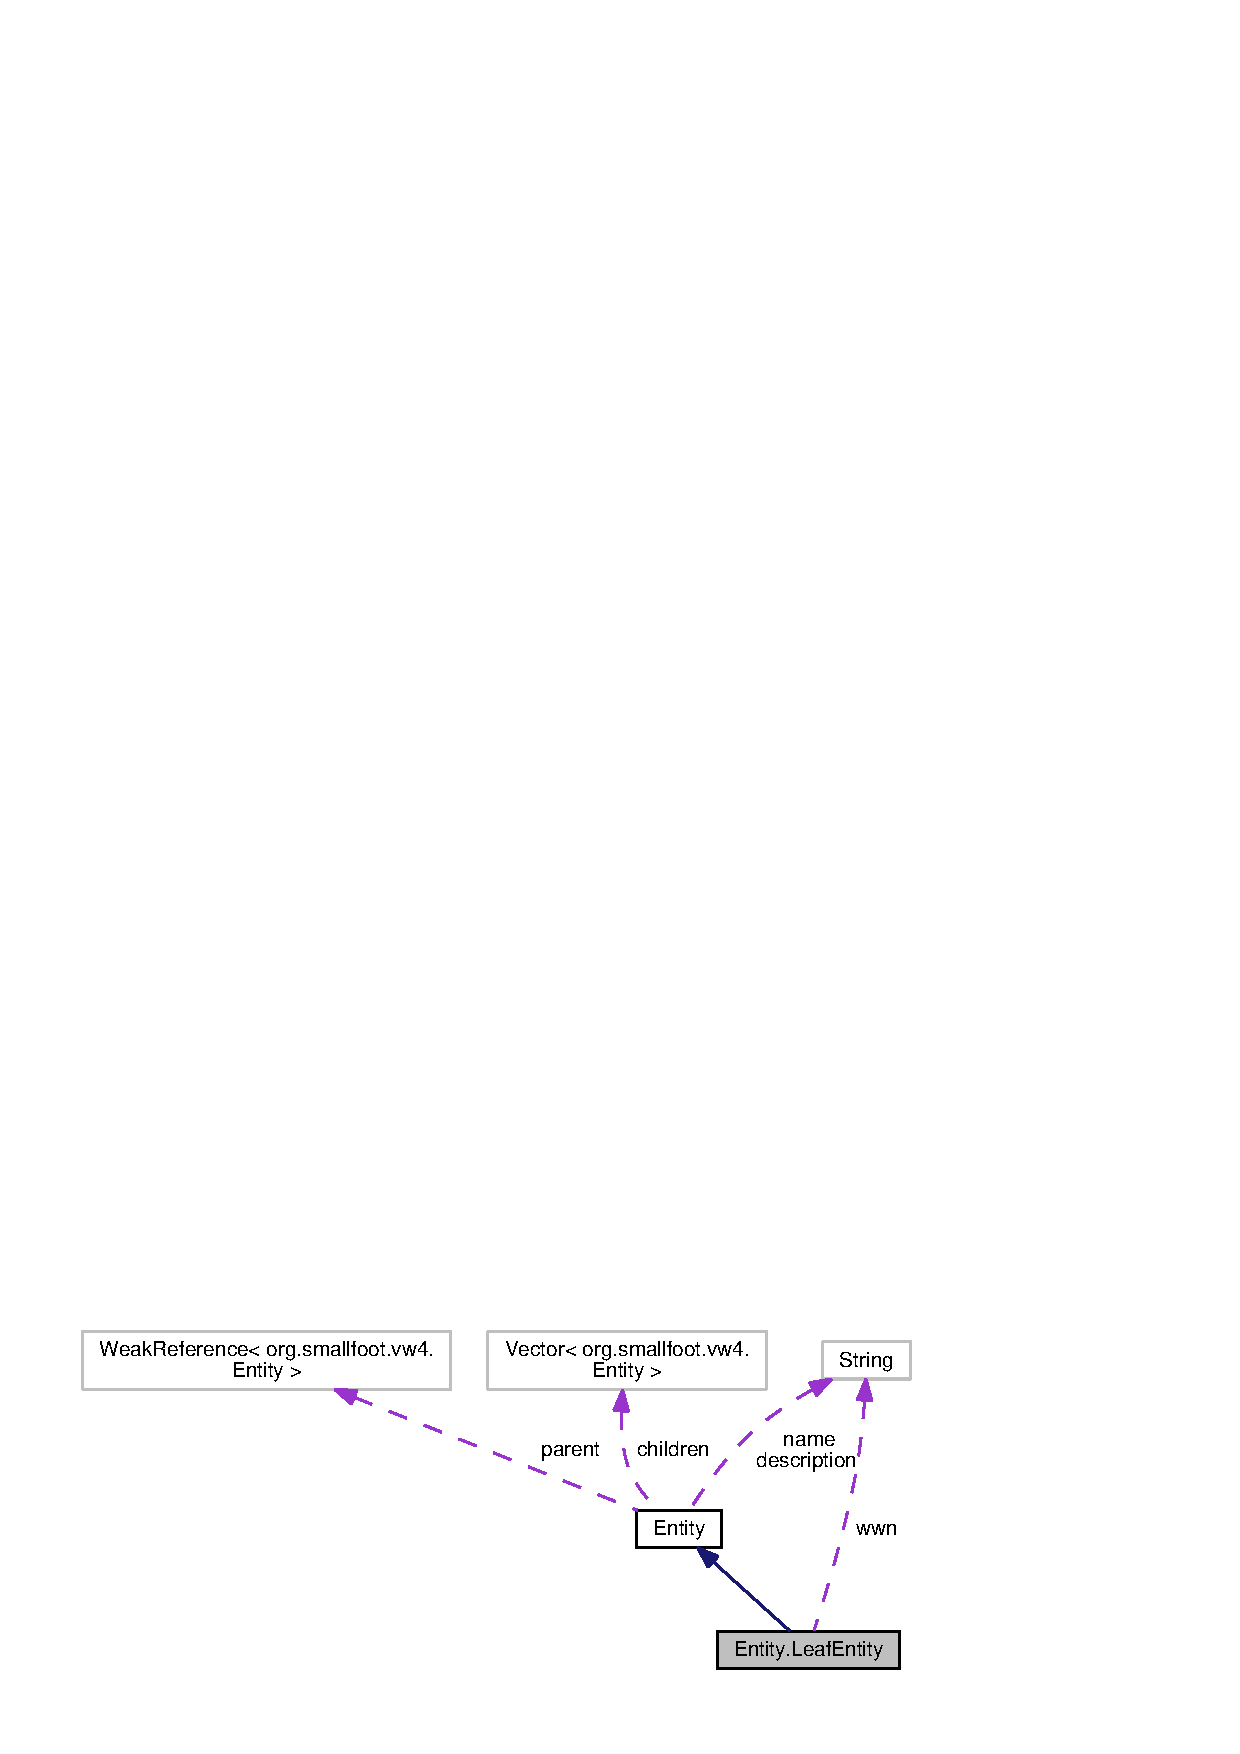
\includegraphics[width=350pt]{classorg_1_1smallfoot_1_1vw4_1_1Entity_1_1LeafEntity__coll__graph}
\end{center}
\end{figure}
\subsection*{Public Member Functions}
\begin{DoxyCompactItemize}
\item 
{\bf Leaf\+Entity} (String {\bf name}, String {\bf wwn})
\begin{DoxyCompactList}\small\item\em Class Constructor with an initial child to absorb. \end{DoxyCompactList}\item 
{\bf Entity} {\bf new\+Parent} (String {\bf name})
\begin{DoxyCompactList}\small\item\em create a new \doxyref{Entity}{p.}{classorg_1_1smallfoot_1_1vw4_1_1Entity} of the correct class to be a parent of this one\+: this function is stubbed to return null so that this class can be a static class and directly extensible. \end{DoxyCompactList}\item 
String {\bf parent\+Name} ()
\begin{DoxyCompactList}\small\item\em convenience function\+: if this entity has a parent, show the parent's name, otherwise show this entity's name. \end{DoxyCompactList}\item 
String {\bf wwn} ()
\begin{DoxyCompactList}\small\item\em the unique W\+W\+P\+N of the hba\+: getter for internal variable \end{DoxyCompactList}\end{DoxyCompactItemize}
\subsection*{Protected Member Functions}
\begin{DoxyCompactItemize}
\item 
boolean {\bf can\+Be\+Child} ({\bf Entity} e)
\begin{DoxyCompactList}\small\item\em whether a given entity can be this entity's child \end{DoxyCompactList}\item 
org.\+smallfoot.\+vw4.\+V\+W\+Import.\+Entity {\bf vwentity} (String tag)\label{classorg_1_1smallfoot_1_1vw4_1_1Entity_1_1LeafEntity_a1d6bf85ddf0a9382cfa4f82dd3063473}

\begin{DoxyCompactList}\small\item\em create a bogus function to avoid build errors \end{DoxyCompactList}\end{DoxyCompactItemize}
\subsection*{Protected Attributes}
\begin{DoxyCompactItemize}
\item 
String {\bf wwn}\label{classorg_1_1smallfoot_1_1vw4_1_1Entity_1_1LeafEntity_ab07f595ad2e4da7c53cd29f435f5bb3c}

\begin{DoxyCompactList}\small\item\em the unique W\+W\+P\+N of the hba \end{DoxyCompactList}\end{DoxyCompactItemize}


\subsection{Detailed Description}
A \doxyref{Leaf\+Entity}{p.}{classorg_1_1smallfoot_1_1vw4_1_1Entity_1_1LeafEntity} is the common ancestor of Storage F\+As and Server H\+B\+As; this is combined only so that leaves can be treated in common. 

Definition at line 202 of file Entity.\+java.



\subsection{Constructor \& Destructor Documentation}
\index{org\+::smallfoot\+::vw4\+::\+Entity\+::\+Leaf\+Entity@{org\+::smallfoot\+::vw4\+::\+Entity\+::\+Leaf\+Entity}!Leaf\+Entity@{Leaf\+Entity}}
\index{Leaf\+Entity@{Leaf\+Entity}!org\+::smallfoot\+::vw4\+::\+Entity\+::\+Leaf\+Entity@{org\+::smallfoot\+::vw4\+::\+Entity\+::\+Leaf\+Entity}}
\subsubsection[{Leaf\+Entity}]{\setlength{\rightskip}{0pt plus 5cm}{\bf Leaf\+Entity} (
\begin{DoxyParamCaption}
\item[{String}]{name, }
\item[{String}]{wwn}
\end{DoxyParamCaption}
)\hspace{0.3cm}{\ttfamily [inline]}}\label{classorg_1_1smallfoot_1_1vw4_1_1Entity_1_1LeafEntity_a30cc6402437a41c9da17a4e50fc9590c}


Class Constructor with an initial child to absorb. 


\begin{DoxyParams}{Parameters}
{\em name} & initial name of the new entity \\
\hline
{\em wwn} & initial child entity for this Leaf \doxyref{Entity}{p.}{classorg_1_1smallfoot_1_1vw4_1_1Entity} \\
\hline
\end{DoxyParams}


Definition at line 233 of file Entity.\+java.



References Entity.\+Leaf\+Entity.\+wwn().



Here is the call graph for this function\+:\nopagebreak
\begin{figure}[H]
\begin{center}
\leavevmode
\includegraphics[width=176pt]{classorg_1_1smallfoot_1_1vw4_1_1Entity_1_1LeafEntity_a30cc6402437a41c9da17a4e50fc9590c_cgraph}
\end{center}
\end{figure}




\subsection{Member Function Documentation}
\index{org\+::smallfoot\+::vw4\+::\+Entity\+::\+Leaf\+Entity@{org\+::smallfoot\+::vw4\+::\+Entity\+::\+Leaf\+Entity}!can\+Be\+Child@{can\+Be\+Child}}
\index{can\+Be\+Child@{can\+Be\+Child}!org\+::smallfoot\+::vw4\+::\+Entity\+::\+Leaf\+Entity@{org\+::smallfoot\+::vw4\+::\+Entity\+::\+Leaf\+Entity}}
\subsubsection[{can\+Be\+Child}]{\setlength{\rightskip}{0pt plus 5cm}boolean can\+Be\+Child (
\begin{DoxyParamCaption}
\item[{{\bf Entity}}]{e}
\end{DoxyParamCaption}
)\hspace{0.3cm}{\ttfamily [inline]}, {\ttfamily [protected]}}\label{classorg_1_1smallfoot_1_1vw4_1_1Entity_1_1LeafEntity_a5a51654ce8be38d5f06faa182cb70e61}


whether a given entity can be this entity's child 

\begin{DoxyReturn}{Returns}
true if accepted, false if refused. \doxyref{Leaf\+Entity}{p.}{classorg_1_1smallfoot_1_1vw4_1_1Entity_1_1LeafEntity} has no children so this method will always be false
\end{DoxyReturn}

\begin{DoxyParams}{Parameters}
{\em e} & entity to check for possible descendent-\/hood \\
\hline
\end{DoxyParams}
\begin{DoxyReturn}{Returns}
true if this entity accepts children of \char`\"{}e\char`\"{}'s descendent type (always false for Leaf \doxyref{Entity}{p.}{classorg_1_1smallfoot_1_1vw4_1_1Entity}) 
\end{DoxyReturn}


Definition at line 246 of file Entity.\+java.

\index{org\+::smallfoot\+::vw4\+::\+Entity\+::\+Leaf\+Entity@{org\+::smallfoot\+::vw4\+::\+Entity\+::\+Leaf\+Entity}!new\+Parent@{new\+Parent}}
\index{new\+Parent@{new\+Parent}!org\+::smallfoot\+::vw4\+::\+Entity\+::\+Leaf\+Entity@{org\+::smallfoot\+::vw4\+::\+Entity\+::\+Leaf\+Entity}}
\subsubsection[{new\+Parent}]{\setlength{\rightskip}{0pt plus 5cm}{\bf Entity} new\+Parent (
\begin{DoxyParamCaption}
\item[{String}]{name}
\end{DoxyParamCaption}
)\hspace{0.3cm}{\ttfamily [inline]}}\label{classorg_1_1smallfoot_1_1vw4_1_1Entity_1_1LeafEntity_ae3cca685b4cef300a70d257f519a96e4}


create a new \doxyref{Entity}{p.}{classorg_1_1smallfoot_1_1vw4_1_1Entity} of the correct class to be a parent of this one\+: this function is stubbed to return null so that this class can be a static class and directly extensible. 

Not really 100\% good practice, but the descendency of this \doxyref{Leaf\+Entity}{p.}{classorg_1_1smallfoot_1_1vw4_1_1Entity_1_1LeafEntity} is intended to collect functionality. This class is wrapped inside an \doxyref{Entity}{p.}{classorg_1_1smallfoot_1_1vw4_1_1Entity} to retain a clear affinity, but thence needs to be static to be extensible. \char`\"{}\+She swallowed the cat to catch the spider, she swallowed the
spider to catch the fly.. \char`\"{}

Descendents will override this method

\begin{DoxyReturn}{Returns}
new parent for this entity 
\end{DoxyReturn}

\begin{DoxyParams}{Parameters}
{\em name} & initial name of the new entity \\
\hline
\end{DoxyParams}


Definition at line 271 of file Entity.\+java.

\index{org\+::smallfoot\+::vw4\+::\+Entity\+::\+Leaf\+Entity@{org\+::smallfoot\+::vw4\+::\+Entity\+::\+Leaf\+Entity}!parent\+Name@{parent\+Name}}
\index{parent\+Name@{parent\+Name}!org\+::smallfoot\+::vw4\+::\+Entity\+::\+Leaf\+Entity@{org\+::smallfoot\+::vw4\+::\+Entity\+::\+Leaf\+Entity}}
\subsubsection[{parent\+Name}]{\setlength{\rightskip}{0pt plus 5cm}String parent\+Name (
\begin{DoxyParamCaption}
{}
\end{DoxyParamCaption}
)\hspace{0.3cm}{\ttfamily [inline]}}\label{classorg_1_1smallfoot_1_1vw4_1_1Entity_1_1LeafEntity_a929a7f5f05728b26869df0351a7a815d}


convenience function\+: if this entity has a parent, show the parent's name, otherwise show this entity's name. 

Used during Ordered\+Tuples written via Virtual\+Wisdom4\+Client\+Tool.\+write\+Ordered\+Tuples(\+String, Entity\+Selector), this allows a simpler, consistent coding when Ordered\+Tuples is being exported.

\begin{DoxyReturn}{Returns}
name of parent entity is existent, otherwise name of this entity 
\end{DoxyReturn}


Definition at line 219 of file Entity.\+java.



References Entity.\+name().



Here is the call graph for this function\+:\nopagebreak
\begin{figure}[H]
\begin{center}
\leavevmode
\includegraphics[width=302pt]{classorg_1_1smallfoot_1_1vw4_1_1Entity_1_1LeafEntity_a929a7f5f05728b26869df0351a7a815d_cgraph}
\end{center}
\end{figure}


\index{org\+::smallfoot\+::vw4\+::\+Entity\+::\+Leaf\+Entity@{org\+::smallfoot\+::vw4\+::\+Entity\+::\+Leaf\+Entity}!wwn@{wwn}}
\index{wwn@{wwn}!org\+::smallfoot\+::vw4\+::\+Entity\+::\+Leaf\+Entity@{org\+::smallfoot\+::vw4\+::\+Entity\+::\+Leaf\+Entity}}
\subsubsection[{wwn}]{\setlength{\rightskip}{0pt plus 5cm}String wwn (
\begin{DoxyParamCaption}
{}
\end{DoxyParamCaption}
)\hspace{0.3cm}{\ttfamily [inline]}}\label{classorg_1_1smallfoot_1_1vw4_1_1Entity_1_1LeafEntity_aa0f20764b2a9bea375e9507de63cb42b}


the unique W\+W\+P\+N of the hba\+: getter for internal variable 

\begin{DoxyReturn}{Returns}
the W\+W\+P\+N 
\end{DoxyReturn}


Definition at line 206 of file Entity.\+java.



Referenced by Entity.\+Leaf\+Entity.\+Leaf\+Entity(), Entity\+H\+B\+A.\+vwentity(), and Entity\+F\+A.\+vwentity().



The documentation for this class was generated from the following file\+:\begin{DoxyCompactItemize}
\item 
java/{\bf Entity.\+java}\end{DoxyCompactItemize}

\section{Virtual\+Wisdom4\+Client\+Tool Class Reference}
\label{classorg_1_1smallfoot_1_1vw4_1_1VirtualWisdom4ClientTool}\index{Virtual\+Wisdom4\+Client\+Tool@{Virtual\+Wisdom4\+Client\+Tool}}


\doxyref{Virtual\+Wisdom4\+Client\+Tool}{p.}{classorg_1_1smallfoot_1_1vw4_1_1VirtualWisdom4ClientTool} is a \char`\"{}\+Swiss Army Knife\char`\"{} of tools used when working with Virtual\+Wisdom4.  




Collaboration diagram for Virtual\+Wisdom4\+Client\+Tool\+:\nopagebreak
\begin{figure}[H]
\begin{center}
\leavevmode
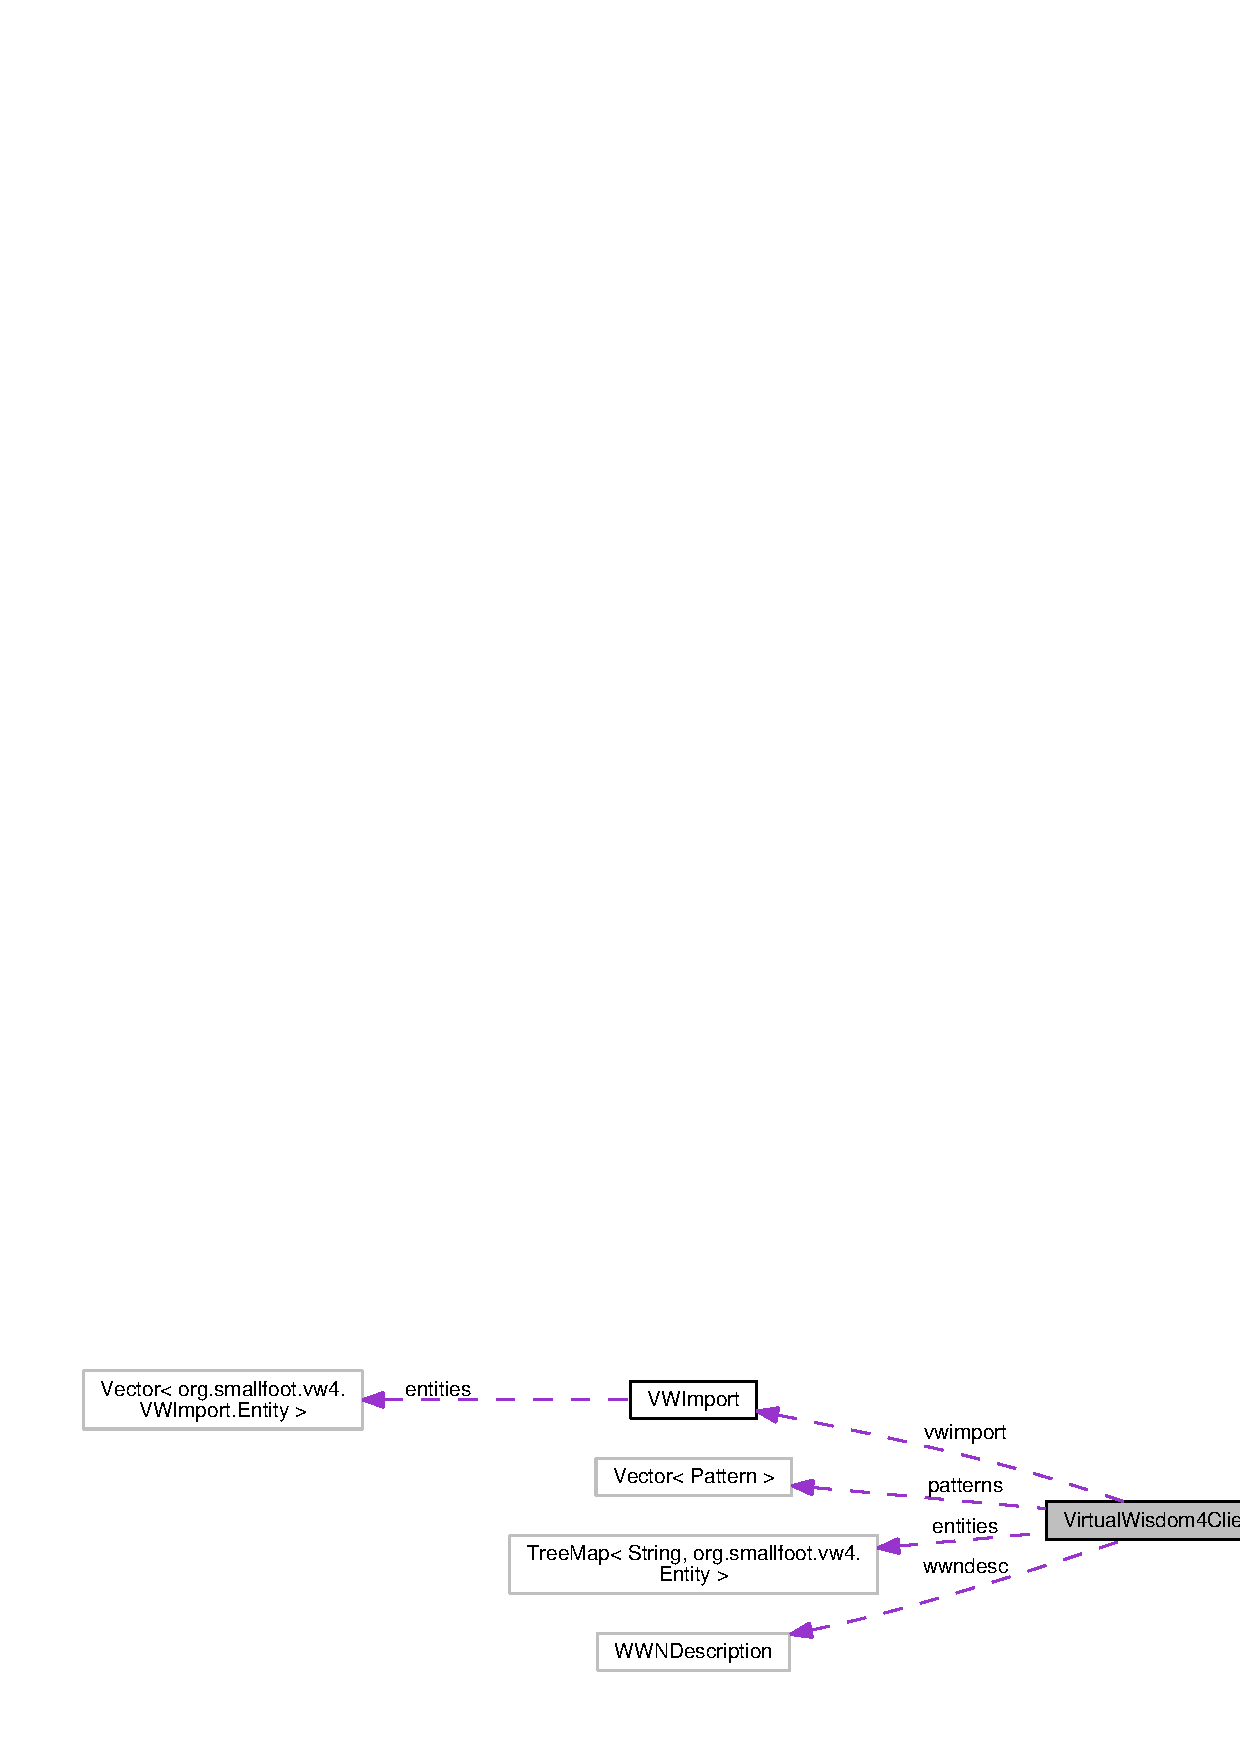
\includegraphics[width=350pt]{classorg_1_1smallfoot_1_1vw4_1_1VirtualWisdom4ClientTool__coll__graph}
\end{center}
\end{figure}
\subsection*{Public Member Functions}
\begin{DoxyCompactItemize}
\item 
{\bf Virtual\+Wisdom4\+Client\+Tool} (String xml\+File)
\begin{DoxyCompactList}\small\item\em Class Constructor to create with an initial file to load. \end{DoxyCompactList}\item 
{\bf Virtual\+Wisdom4\+Client\+Tool} ()\label{classorg_1_1smallfoot_1_1vw4_1_1VirtualWisdom4ClientTool_a7991b30b52ad4d408df3575abc9b57ae}

\begin{DoxyCompactList}\small\item\em Class Constructor with no initial file. \end{DoxyCompactList}\item 
Tree\+Map$<$ String, {\bf Entity} $>$ {\bf entities} ()
\item 
void {\bf load} (String filename)
\begin{DoxyCompactList}\small\item\em Wrapper to just load the file, spitting out exceptions and stacks as they occur. \end{DoxyCompactList}\item 
Vector$<$ Pattern $>$ {\bf patterns} ()
\item 
String {\bf pretty\+J\+S\+O\+N} (V\+W\+Import v)
\begin{DoxyCompactList}\small\item\em Convenience function to generate a pretty-\/printed J\+S\+O\+N text string. \end{DoxyCompactList}\item 
void {\bf save} (String filename)
\begin{DoxyCompactList}\small\item\em Wrapper to just save the file, spitting out exceptions and stacks as they occur. \end{DoxyCompactList}\item 
W\+W\+N\+Description {\bf wwndesc} ()
\end{DoxyCompactItemize}
\subsection*{Static Public Member Functions}
\begin{DoxyCompactItemize}
\item 
static void {\bf main} (String args[$\,$])
\begin{DoxyCompactList}\small\item\em Main function, as you can tell. \end{DoxyCompactList}\end{DoxyCompactItemize}
\subsection*{Data Fields}
\begin{DoxyCompactItemize}
\item 
V\+W\+Import {\bf vwimport} = null\label{classorg_1_1smallfoot_1_1vw4_1_1VirtualWisdom4ClientTool_a4ef055893be8838f513385e4c2f42700}

\begin{DoxyCompactList}\small\item\em singleton list of J\+S\+O\+N-\/writable objects accessed through \doxyref{vwimport()}{p.}{classorg_1_1smallfoot_1_1vw4_1_1VirtualWisdom4ClientTool_acbeee875159f78e186965708e70dee94} \end{DoxyCompactList}\end{DoxyCompactItemize}
\subsection*{Protected Member Functions}
\begin{DoxyCompactItemize}
\item 
void {\bf \+\_\+load} (String filename)  throws java.\+io.\+I\+O\+Exception     
\begin{DoxyCompactList}\small\item\em Open a file. \end{DoxyCompactList}\item 
void {\bf \+\_\+save} (String filename)  throws java.\+lang.\+Exception     
\begin{DoxyCompactList}\small\item\em Save the current X\+M\+L Document to a new file. \end{DoxyCompactList}\item 
void {\bf load\+And\+Absorb\+File} (String f)
\begin{DoxyCompactList}\small\item\em one-\/shot load a new file and absorb the contents\+: open the file and stream the contents at an array of parsers, the one with the best results wins; using that result, absorb all alias information, attempting to create parent storagecontroller(s) or hosts as resulting from absorbtion patterns \end{DoxyCompactList}\item 
void {\bf load\+And\+Remove\+File} (String f)
\begin{DoxyCompactList}\small\item\em one-\/shot load a new file and remove the contents from the internal list of leaf\+Entities (H\+B\+As, F\+As) \end{DoxyCompactList}\item 
V\+W\+Import {\bf vwimport} ()
\end{DoxyCompactItemize}
\subsection*{Protected Attributes}
\begin{DoxyCompactItemize}
\item 
Tree\+Map$<$ String, {\bf Entity} $>$ {\bf entities} = null\label{classorg_1_1smallfoot_1_1vw4_1_1VirtualWisdom4ClientTool_ac3c495e48cdbca229137371be08ba04f}

\begin{DoxyCompactList}\small\item\em local singleton array accessed from \doxyref{entities()}{p.}{classorg_1_1smallfoot_1_1vw4_1_1VirtualWisdom4ClientTool_aa9ab77e799e869cf9da3d339e124f6c4} \end{DoxyCompactList}\item 
Vector$<$ Pattern $>$ {\bf patterns} = null\label{classorg_1_1smallfoot_1_1vw4_1_1VirtualWisdom4ClientTool_aaa7580a75c1bf3c122ce5b4c001517c2}

\begin{DoxyCompactList}\small\item\em local singleton array accessed from \doxyref{patterns()}{p.}{classorg_1_1smallfoot_1_1vw4_1_1VirtualWisdom4ClientTool_a09f298d19a33be899f5835657c747c5d} \end{DoxyCompactList}\item 
W\+W\+N\+Description {\bf wwndesc} = null\label{classorg_1_1smallfoot_1_1vw4_1_1VirtualWisdom4ClientTool_afb3f7acf97044713e2aa55c921c5cdb2}

\begin{DoxyCompactList}\small\item\em local singleton array accessed from \doxyref{wwndesc()}{p.}{classorg_1_1smallfoot_1_1vw4_1_1VirtualWisdom4ClientTool_a43a8de962936ee9d82e0a70eeb9b1db6} \end{DoxyCompactList}\end{DoxyCompactItemize}
\subsection*{Private Attributes}
\begin{DoxyCompactItemize}
\item 
org.\+w3c.\+dom.\+Document {\bf xml\+Document}\label{classorg_1_1smallfoot_1_1vw4_1_1VirtualWisdom4ClientTool_ad25ef6220eb54575157ab063bc63a0f0}

\begin{DoxyCompactList}\small\item\em eventually used to hold an X\+M\+L document when converting X\+M\+L$<$--$>$J\+S\+O\+N$<$--$>$X\+M\+L \end{DoxyCompactList}\end{DoxyCompactItemize}


\subsection{Detailed Description}
\doxyref{Virtual\+Wisdom4\+Client\+Tool}{p.}{classorg_1_1smallfoot_1_1vw4_1_1VirtualWisdom4ClientTool} is a \char`\"{}\+Swiss Army Knife\char`\"{} of tools used when working with Virtual\+Wisdom4. 

The existence of these tools is not a judgement on Virtual\+Wisdom4's proper Engineering; rather, an acceptance that a faster-\/response solution for the longer-\/tail of the normal curve is often helpful swapping Q\+A delay for reduced customer friction.

As you'd expect, there is no support for this. If it breaks, you may choose to keep both pieces \+:)

Ad-\/\+Hoc content for this utility-\/stack may appear at {\tt http\+://fcfae.\+com/} 

Definition at line 56 of file Virtual\+Wisdom4\+Client\+Tool.\+java.



\subsection{Constructor \& Destructor Documentation}
\index{org\+::smallfoot\+::vw4\+::\+Virtual\+Wisdom4\+Client\+Tool@{org\+::smallfoot\+::vw4\+::\+Virtual\+Wisdom4\+Client\+Tool}!Virtual\+Wisdom4\+Client\+Tool@{Virtual\+Wisdom4\+Client\+Tool}}
\index{Virtual\+Wisdom4\+Client\+Tool@{Virtual\+Wisdom4\+Client\+Tool}!org\+::smallfoot\+::vw4\+::\+Virtual\+Wisdom4\+Client\+Tool@{org\+::smallfoot\+::vw4\+::\+Virtual\+Wisdom4\+Client\+Tool}}
\subsubsection[{Virtual\+Wisdom4\+Client\+Tool}]{\setlength{\rightskip}{0pt plus 5cm}{\bf Virtual\+Wisdom4\+Client\+Tool} (
\begin{DoxyParamCaption}
\item[{String}]{xml\+File}
\end{DoxyParamCaption}
)\hspace{0.3cm}{\ttfamily [inline]}}\label{classorg_1_1smallfoot_1_1vw4_1_1VirtualWisdom4ClientTool_a0f1b4c518fafff8a296bb632e57655ca}


Class Constructor to create with an initial file to load. 


\begin{DoxyParams}{Parameters}
{\em xml\+File} & File to load at start\\
\hline
\end{DoxyParams}
\begin{DoxySeeAlso}{See also}
\doxyref{load(\+String)}{p.}{classorg_1_1smallfoot_1_1vw4_1_1VirtualWisdom4ClientTool_a0d686f1044a2e8727b12e6e4921e0e8f} 
\end{DoxySeeAlso}


Definition at line 67 of file Virtual\+Wisdom4\+Client\+Tool.\+java.



References Virtual\+Wisdom4\+Client\+Tool.\+load().



Here is the call graph for this function\+:\nopagebreak
\begin{figure}[H]
\begin{center}
\leavevmode
\includegraphics[width=322pt]{classorg_1_1smallfoot_1_1vw4_1_1VirtualWisdom4ClientTool_a0f1b4c518fafff8a296bb632e57655ca_cgraph}
\end{center}
\end{figure}




\subsection{Member Function Documentation}
\index{org\+::smallfoot\+::vw4\+::\+Virtual\+Wisdom4\+Client\+Tool@{org\+::smallfoot\+::vw4\+::\+Virtual\+Wisdom4\+Client\+Tool}!\+\_\+load@{\+\_\+load}}
\index{\+\_\+load@{\+\_\+load}!org\+::smallfoot\+::vw4\+::\+Virtual\+Wisdom4\+Client\+Tool@{org\+::smallfoot\+::vw4\+::\+Virtual\+Wisdom4\+Client\+Tool}}
\subsubsection[{\+\_\+load}]{\setlength{\rightskip}{0pt plus 5cm}void \+\_\+load (
\begin{DoxyParamCaption}
\item[{String}]{filename}
\end{DoxyParamCaption}
) throws java.\+io.\+I\+O\+Exception\hspace{0.3cm}{\ttfamily [inline]}, {\ttfamily [protected]}}\label{classorg_1_1smallfoot_1_1vw4_1_1VirtualWisdom4ClientTool_ad9a051ba608e7fcb9adac39bc3946058}


Open a file. 

This is actually a wrapper for the underlying file load


\begin{DoxyParams}{Parameters}
{\em filename} & file to load \\
\hline
\end{DoxyParams}

\begin{DoxyExceptions}{Exceptions}
{\em I\+O\+Exception} & when File() encounters an error instaitating (typically path or permissions) \\
\hline
\end{DoxyExceptions}
\begin{DoxyRefDesc}{Todo}
\item[{\bf Todo}]\+: evaluate\+: mapper.\+configure(Deserialization\+Config.\+Feature.\+F\+A\+I\+L\+\_\+\+O\+N\+\_\+\+U\+N\+K\+N\+O\+W\+N\+\_\+\+P\+R\+O\+P\+E\+R\+T\+I\+E\+S, false); \end{DoxyRefDesc}


Definition at line 96 of file Virtual\+Wisdom4\+Client\+Tool.\+java.



Referenced by Virtual\+Wisdom4\+Client\+Tool.\+load().

\index{org\+::smallfoot\+::vw4\+::\+Virtual\+Wisdom4\+Client\+Tool@{org\+::smallfoot\+::vw4\+::\+Virtual\+Wisdom4\+Client\+Tool}!\+\_\+save@{\+\_\+save}}
\index{\+\_\+save@{\+\_\+save}!org\+::smallfoot\+::vw4\+::\+Virtual\+Wisdom4\+Client\+Tool@{org\+::smallfoot\+::vw4\+::\+Virtual\+Wisdom4\+Client\+Tool}}
\subsubsection[{\+\_\+save}]{\setlength{\rightskip}{0pt plus 5cm}void \+\_\+save (
\begin{DoxyParamCaption}
\item[{String}]{filename}
\end{DoxyParamCaption}
) throws java.\+lang.\+Exception\hspace{0.3cm}{\ttfamily [inline]}, {\ttfamily [protected]}}\label{classorg_1_1smallfoot_1_1vw4_1_1VirtualWisdom4ClientTool_a36a7decd28b5e191bfe43c5562462785}


Save the current X\+M\+L Document to a new file. 


\begin{DoxyParams}{Parameters}
{\em filename} & filename to save into \\
\hline
\end{DoxyParams}


Definition at line 131 of file Virtual\+Wisdom4\+Client\+Tool.\+java.



Referenced by Virtual\+Wisdom4\+Client\+Tool.\+save().

\index{org\+::smallfoot\+::vw4\+::\+Virtual\+Wisdom4\+Client\+Tool@{org\+::smallfoot\+::vw4\+::\+Virtual\+Wisdom4\+Client\+Tool}!entities@{entities}}
\index{entities@{entities}!org\+::smallfoot\+::vw4\+::\+Virtual\+Wisdom4\+Client\+Tool@{org\+::smallfoot\+::vw4\+::\+Virtual\+Wisdom4\+Client\+Tool}}
\subsubsection[{entities}]{\setlength{\rightskip}{0pt plus 5cm}Tree\+Map$<$String,{\bf Entity}$>$ entities (
\begin{DoxyParamCaption}
{}
\end{DoxyParamCaption}
)\hspace{0.3cm}{\ttfamily [inline]}}\label{classorg_1_1smallfoot_1_1vw4_1_1VirtualWisdom4ClientTool_aa9ab77e799e869cf9da3d339e124f6c4}
$<$ singleton access for entities \begin{DoxyReturn}{Returns}
collection of entities 
\end{DoxyReturn}


Definition at line 194 of file Virtual\+Wisdom4\+Client\+Tool.\+java.



Referenced by Virtual\+Wisdom4\+Client\+Tool.\+load\+And\+Absorb\+File().

\index{org\+::smallfoot\+::vw4\+::\+Virtual\+Wisdom4\+Client\+Tool@{org\+::smallfoot\+::vw4\+::\+Virtual\+Wisdom4\+Client\+Tool}!load@{load}}
\index{load@{load}!org\+::smallfoot\+::vw4\+::\+Virtual\+Wisdom4\+Client\+Tool@{org\+::smallfoot\+::vw4\+::\+Virtual\+Wisdom4\+Client\+Tool}}
\subsubsection[{load}]{\setlength{\rightskip}{0pt plus 5cm}void load (
\begin{DoxyParamCaption}
\item[{String}]{filename}
\end{DoxyParamCaption}
)\hspace{0.3cm}{\ttfamily [inline]}}\label{classorg_1_1smallfoot_1_1vw4_1_1VirtualWisdom4ClientTool_a0d686f1044a2e8727b12e6e4921e0e8f}


Wrapper to just load the file, spitting out exceptions and stacks as they occur. 


\begin{DoxyParams}{Parameters}
{\em filename} & file to load \\
\hline
\end{DoxyParams}


Definition at line 110 of file Virtual\+Wisdom4\+Client\+Tool.\+java.



References Virtual\+Wisdom4\+Client\+Tool.\+\_\+load().



Referenced by Virtual\+Wisdom4\+Client\+Tool.\+main(), and Virtual\+Wisdom4\+Client\+Tool.\+Virtual\+Wisdom4\+Client\+Tool().



Here is the call graph for this function\+:\nopagebreak
\begin{figure}[H]
\begin{center}
\leavevmode
\includegraphics[width=156pt]{classorg_1_1smallfoot_1_1vw4_1_1VirtualWisdom4ClientTool_a0d686f1044a2e8727b12e6e4921e0e8f_cgraph}
\end{center}
\end{figure}


\index{org\+::smallfoot\+::vw4\+::\+Virtual\+Wisdom4\+Client\+Tool@{org\+::smallfoot\+::vw4\+::\+Virtual\+Wisdom4\+Client\+Tool}!load\+And\+Absorb\+File@{load\+And\+Absorb\+File}}
\index{load\+And\+Absorb\+File@{load\+And\+Absorb\+File}!org\+::smallfoot\+::vw4\+::\+Virtual\+Wisdom4\+Client\+Tool@{org\+::smallfoot\+::vw4\+::\+Virtual\+Wisdom4\+Client\+Tool}}
\subsubsection[{load\+And\+Absorb\+File}]{\setlength{\rightskip}{0pt plus 5cm}void load\+And\+Absorb\+File (
\begin{DoxyParamCaption}
\item[{String}]{f}
\end{DoxyParamCaption}
)\hspace{0.3cm}{\ttfamily [inline]}, {\ttfamily [protected]}}\label{classorg_1_1smallfoot_1_1vw4_1_1VirtualWisdom4ClientTool_a36539eb2d98fcdcedd7dc2088acfeef2}


one-\/shot load a new file and absorb the contents\+: open the file and stream the contents at an array of parsers, the one with the best results wins; using that result, absorb all alias information, attempting to create parent storagecontroller(s) or hosts as resulting from absorbtion patterns 


\begin{DoxyParams}{Parameters}
{\em f} & name of file to open\\
\hline
\end{DoxyParams}
\begin{DoxySeeAlso}{See also}
{\tt https\+://github.\+com/chickenandpork/fibrechannel-\/parsers/} 
\end{DoxySeeAlso}


Definition at line 345 of file Virtual\+Wisdom4\+Client\+Tool.\+java.



References Virtual\+Wisdom4\+Client\+Tool.\+entities(), Entity.\+name, Virtual\+Wisdom4\+Client\+Tool.\+patterns(), Entity.\+set\+Description(), Entity.\+setname(), and Virtual\+Wisdom4\+Client\+Tool.\+wwndesc().



Referenced by Virtual\+Wisdom4\+Client\+Tool.\+main().



Here is the call graph for this function\+:\nopagebreak
\begin{figure}[H]
\begin{center}
\leavevmode
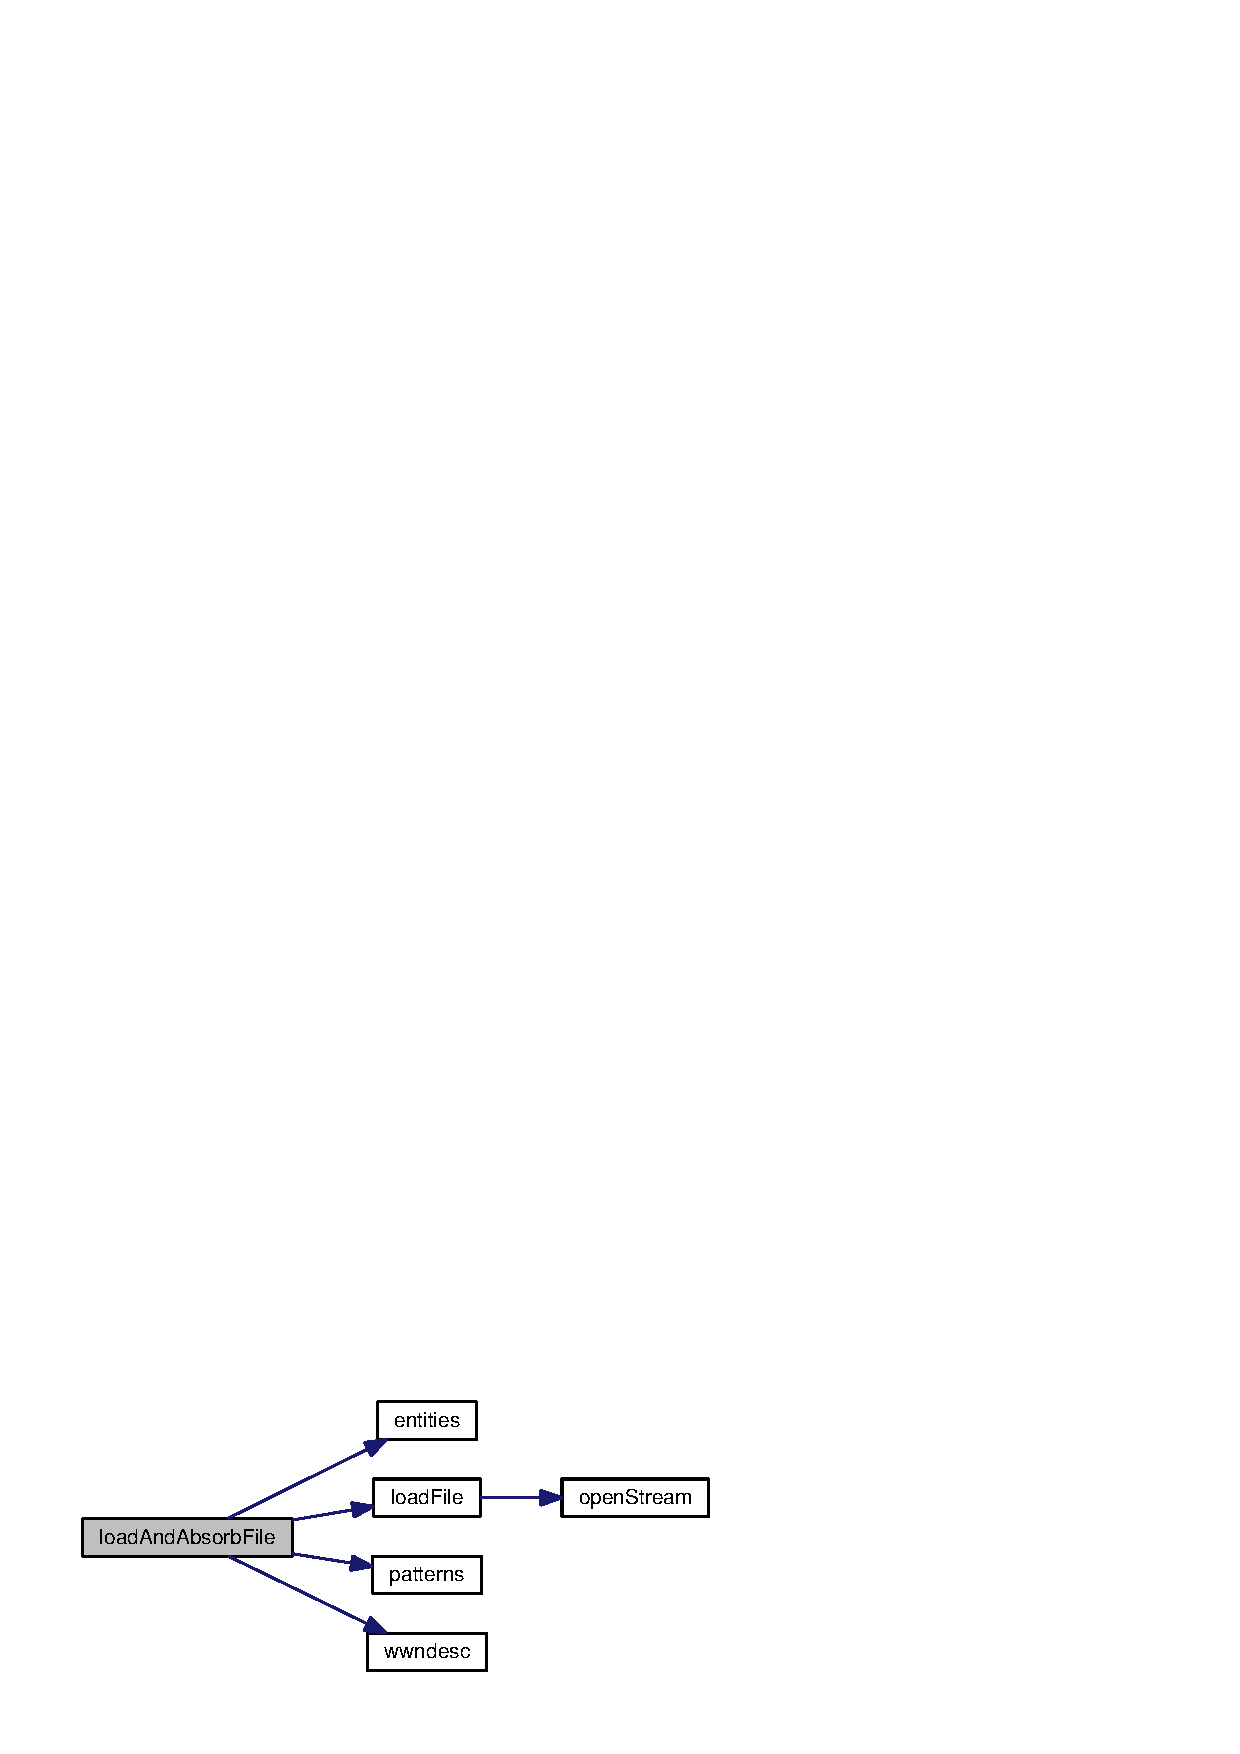
\includegraphics[width=350pt]{classorg_1_1smallfoot_1_1vw4_1_1VirtualWisdom4ClientTool_a36539eb2d98fcdcedd7dc2088acfeef2_cgraph}
\end{center}
\end{figure}


\index{org\+::smallfoot\+::vw4\+::\+Virtual\+Wisdom4\+Client\+Tool@{org\+::smallfoot\+::vw4\+::\+Virtual\+Wisdom4\+Client\+Tool}!load\+And\+Remove\+File@{load\+And\+Remove\+File}}
\index{load\+And\+Remove\+File@{load\+And\+Remove\+File}!org\+::smallfoot\+::vw4\+::\+Virtual\+Wisdom4\+Client\+Tool@{org\+::smallfoot\+::vw4\+::\+Virtual\+Wisdom4\+Client\+Tool}}
\subsubsection[{load\+And\+Remove\+File}]{\setlength{\rightskip}{0pt plus 5cm}void load\+And\+Remove\+File (
\begin{DoxyParamCaption}
\item[{String}]{f}
\end{DoxyParamCaption}
)\hspace{0.3cm}{\ttfamily [inline]}, {\ttfamily [protected]}}\label{classorg_1_1smallfoot_1_1vw4_1_1VirtualWisdom4ClientTool_a2e5ab2ec8715ec815edcea74375a493c}


one-\/shot load a new file and remove the contents from the internal list of leaf\+Entities (H\+B\+As, F\+As) 

Working on only the leaf entities, this uses the parser array to parse an input stream, and for each W\+W\+P\+N found, it removes that leaf entity from the system. It doesn't affect the child\+\_\+entities of referring entities to allow for a loaded entity list to still refer to entities which are already on the target system.


\begin{DoxyParams}{Parameters}
{\em f} & name of file to open\\
\hline
\end{DoxyParams}
\begin{DoxySeeAlso}{See also}
{\tt https\+://github.\+com/chickenandpork/fibrechannel-\/parsers/} 
\end{DoxySeeAlso}


Definition at line 284 of file Virtual\+Wisdom4\+Client\+Tool.\+java.



Referenced by Virtual\+Wisdom4\+Client\+Tool.\+main().

\index{org\+::smallfoot\+::vw4\+::\+Virtual\+Wisdom4\+Client\+Tool@{org\+::smallfoot\+::vw4\+::\+Virtual\+Wisdom4\+Client\+Tool}!main@{main}}
\index{main@{main}!org\+::smallfoot\+::vw4\+::\+Virtual\+Wisdom4\+Client\+Tool@{org\+::smallfoot\+::vw4\+::\+Virtual\+Wisdom4\+Client\+Tool}}
\subsubsection[{main}]{\setlength{\rightskip}{0pt plus 5cm}static void main (
\begin{DoxyParamCaption}
\item[{String}]{args[$\,$]}
\end{DoxyParamCaption}
)\hspace{0.3cm}{\ttfamily [inline]}, {\ttfamily [static]}}\label{classorg_1_1smallfoot_1_1vw4_1_1VirtualWisdom4ClientTool_a75988cf84fc6ee7a2ebff36e363021aa}


Main function, as you can tell. 

this function merely parses the command-\/line to dispatch actions to the meat of the meal above. I'm using an actual Get\+Opt because, yes, I'm a U\+N\+I\+X/\+C hack, re-\/using 3-\/decades-\/old knowledge, but this also preserves both extensibility and the ability to use longopts in scripts as a way to self-\/document what the tool's doing.

No real intelligence herein except the parse-\/and-\/redirect action.


\begin{DoxyParams}{Parameters}
{\em args} & as you'd expect, these are commandline arguments given when the jar is activated \\
\hline
\end{DoxyParams}


Definition at line 574 of file Virtual\+Wisdom4\+Client\+Tool.\+java.



References Entity.\+description, Virtual\+Wisdom4\+Client\+Tool.\+entities, Virtual\+Wisdom4\+Client\+Tool.\+load(), Virtual\+Wisdom4\+Client\+Tool.\+load\+And\+Absorb\+File(), Virtual\+Wisdom4\+Client\+Tool.\+load\+And\+Remove\+File(), Entity.\+name, Virtual\+Wisdom4\+Client\+Tool.\+Virtual\+Wisdom4\+Client\+Tool(), and Virtual\+Wisdom4\+Client\+Tool.\+vwimport.



Here is the call graph for this function\+:\nopagebreak
\begin{figure}[H]
\begin{center}
\leavevmode
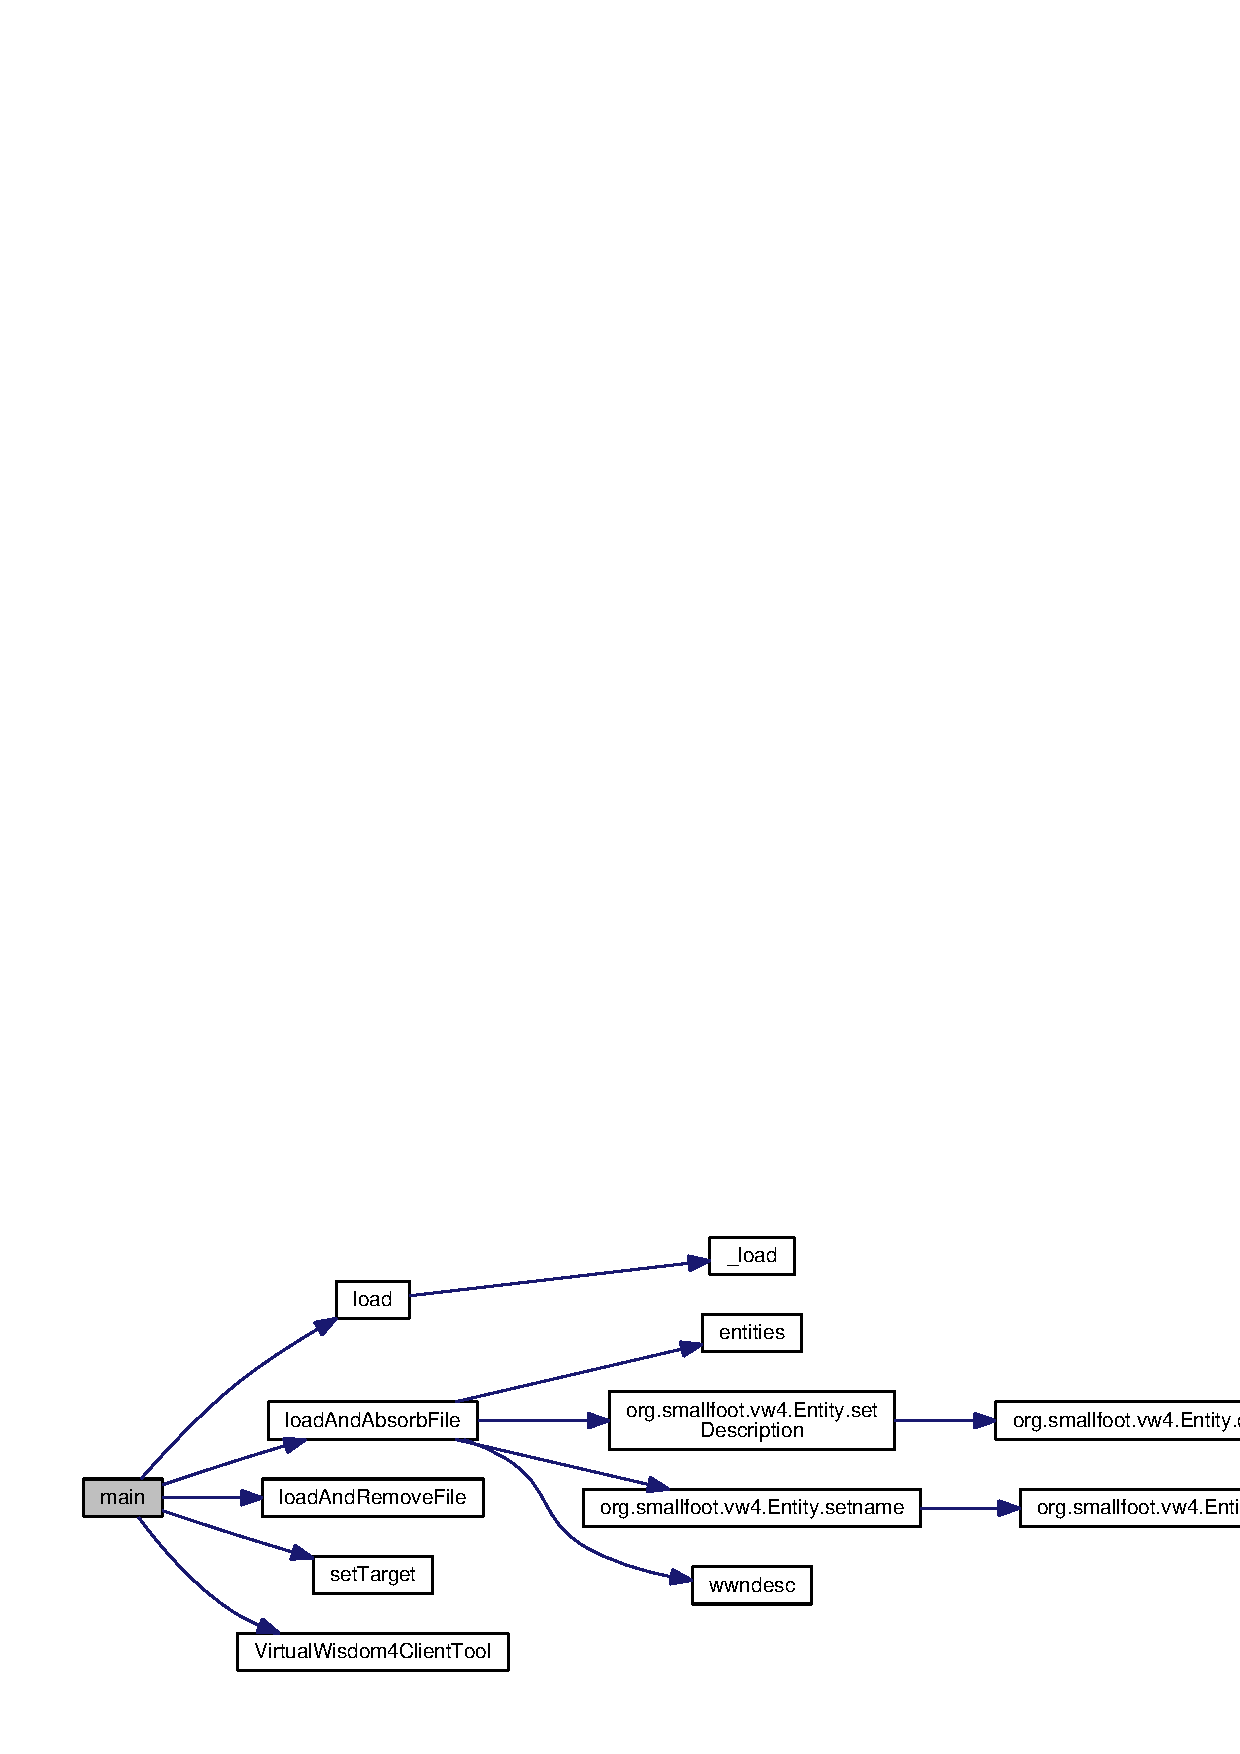
\includegraphics[width=350pt]{classorg_1_1smallfoot_1_1vw4_1_1VirtualWisdom4ClientTool_a75988cf84fc6ee7a2ebff36e363021aa_cgraph}
\end{center}
\end{figure}


\index{org\+::smallfoot\+::vw4\+::\+Virtual\+Wisdom4\+Client\+Tool@{org\+::smallfoot\+::vw4\+::\+Virtual\+Wisdom4\+Client\+Tool}!patterns@{patterns}}
\index{patterns@{patterns}!org\+::smallfoot\+::vw4\+::\+Virtual\+Wisdom4\+Client\+Tool@{org\+::smallfoot\+::vw4\+::\+Virtual\+Wisdom4\+Client\+Tool}}
\subsubsection[{patterns}]{\setlength{\rightskip}{0pt plus 5cm}Vector$<$Pattern$>$ patterns (
\begin{DoxyParamCaption}
{}
\end{DoxyParamCaption}
)\hspace{0.3cm}{\ttfamily [inline]}}\label{classorg_1_1smallfoot_1_1vw4_1_1VirtualWisdom4ClientTool_a09f298d19a33be899f5835657c747c5d}
$<$ singleton access for patterns \begin{DoxyReturn}{Returns}
collection of patterns 
\end{DoxyReturn}


Definition at line 187 of file Virtual\+Wisdom4\+Client\+Tool.\+java.



Referenced by Virtual\+Wisdom4\+Client\+Tool.\+load\+And\+Absorb\+File().

\index{org\+::smallfoot\+::vw4\+::\+Virtual\+Wisdom4\+Client\+Tool@{org\+::smallfoot\+::vw4\+::\+Virtual\+Wisdom4\+Client\+Tool}!pretty\+J\+S\+O\+N@{pretty\+J\+S\+O\+N}}
\index{pretty\+J\+S\+O\+N@{pretty\+J\+S\+O\+N}!org\+::smallfoot\+::vw4\+::\+Virtual\+Wisdom4\+Client\+Tool@{org\+::smallfoot\+::vw4\+::\+Virtual\+Wisdom4\+Client\+Tool}}
\subsubsection[{pretty\+J\+S\+O\+N}]{\setlength{\rightskip}{0pt plus 5cm}String pretty\+J\+S\+O\+N (
\begin{DoxyParamCaption}
\item[{V\+W\+Import}]{v}
\end{DoxyParamCaption}
)\hspace{0.3cm}{\ttfamily [inline]}}\label{classorg_1_1smallfoot_1_1vw4_1_1VirtualWisdom4ClientTool_afc3ee9b897e0757b6cd5c8289c9d4cc4}


Convenience function to generate a pretty-\/printed J\+S\+O\+N text string. 


\begin{DoxyParams}{Parameters}
{\em v} & V\+W\+Import object to markup \\
\hline
\end{DoxyParams}
\begin{DoxyReturn}{Returns}
a pretty-\/printed J\+S\+O\+N using Object\+Writer.\+with\+Default\+Pretty\+Printer() or null if an exception occurs 
\end{DoxyReturn}


Definition at line 161 of file Virtual\+Wisdom4\+Client\+Tool.\+java.

\index{org\+::smallfoot\+::vw4\+::\+Virtual\+Wisdom4\+Client\+Tool@{org\+::smallfoot\+::vw4\+::\+Virtual\+Wisdom4\+Client\+Tool}!save@{save}}
\index{save@{save}!org\+::smallfoot\+::vw4\+::\+Virtual\+Wisdom4\+Client\+Tool@{org\+::smallfoot\+::vw4\+::\+Virtual\+Wisdom4\+Client\+Tool}}
\subsubsection[{save}]{\setlength{\rightskip}{0pt plus 5cm}void save (
\begin{DoxyParamCaption}
\item[{String}]{filename}
\end{DoxyParamCaption}
)\hspace{0.3cm}{\ttfamily [inline]}}\label{classorg_1_1smallfoot_1_1vw4_1_1VirtualWisdom4ClientTool_a119573b242d96a5e64a7d340bcf14aa8}


Wrapper to just save the file, spitting out exceptions and stacks as they occur. 


\begin{DoxyParams}{Parameters}
{\em filename} & filename to save into \\
\hline
\end{DoxyParams}


Definition at line 142 of file Virtual\+Wisdom4\+Client\+Tool.\+java.



References Virtual\+Wisdom4\+Client\+Tool.\+\_\+save().



Here is the call graph for this function\+:\nopagebreak
\begin{figure}[H]
\begin{center}
\leavevmode
\includegraphics[width=162pt]{classorg_1_1smallfoot_1_1vw4_1_1VirtualWisdom4ClientTool_a119573b242d96a5e64a7d340bcf14aa8_cgraph}
\end{center}
\end{figure}


\index{org\+::smallfoot\+::vw4\+::\+Virtual\+Wisdom4\+Client\+Tool@{org\+::smallfoot\+::vw4\+::\+Virtual\+Wisdom4\+Client\+Tool}!vwimport@{vwimport}}
\index{vwimport@{vwimport}!org\+::smallfoot\+::vw4\+::\+Virtual\+Wisdom4\+Client\+Tool@{org\+::smallfoot\+::vw4\+::\+Virtual\+Wisdom4\+Client\+Tool}}
\subsubsection[{vwimport}]{\setlength{\rightskip}{0pt plus 5cm}V\+W\+Import vwimport (
\begin{DoxyParamCaption}
{}
\end{DoxyParamCaption}
)\hspace{0.3cm}{\ttfamily [inline]}, {\ttfamily [protected]}}\label{classorg_1_1smallfoot_1_1vw4_1_1VirtualWisdom4ClientTool_acbeee875159f78e186965708e70dee94}
$<$ singleton to access vwimport to allow for later post-\/process 

Definition at line 82 of file Virtual\+Wisdom4\+Client\+Tool.\+java.



Referenced by Virtual\+Wisdom4\+Client\+Tool.\+main().

\index{org\+::smallfoot\+::vw4\+::\+Virtual\+Wisdom4\+Client\+Tool@{org\+::smallfoot\+::vw4\+::\+Virtual\+Wisdom4\+Client\+Tool}!wwndesc@{wwndesc}}
\index{wwndesc@{wwndesc}!org\+::smallfoot\+::vw4\+::\+Virtual\+Wisdom4\+Client\+Tool@{org\+::smallfoot\+::vw4\+::\+Virtual\+Wisdom4\+Client\+Tool}}
\subsubsection[{wwndesc}]{\setlength{\rightskip}{0pt plus 5cm}W\+W\+N\+Description wwndesc (
\begin{DoxyParamCaption}
{}
\end{DoxyParamCaption}
)\hspace{0.3cm}{\ttfamily [inline]}}\label{classorg_1_1smallfoot_1_1vw4_1_1VirtualWisdom4ClientTool_a43a8de962936ee9d82e0a70eeb9b1db6}
$<$ singleton access for wwndesc \begin{DoxyReturn}{Returns}
wwndesc 
\end{DoxyReturn}


Definition at line 201 of file Virtual\+Wisdom4\+Client\+Tool.\+java.



Referenced by Virtual\+Wisdom4\+Client\+Tool.\+load\+And\+Absorb\+File().



The documentation for this class was generated from the following file\+:\begin{DoxyCompactItemize}
\item 
java/{\bf Virtual\+Wisdom4\+Client\+Tool.\+java}\end{DoxyCompactItemize}

\chapter{File Documentation}
\section{htdocs/\+R\+E\+A\+D\+M\+E.dox File Reference}
\label{README_8dox}\index{htdocs/\+R\+E\+A\+D\+M\+E.\+dox@{htdocs/\+R\+E\+A\+D\+M\+E.\+dox}}


\subsection{Detailed Description}
\subsection*{Building }

This project is a basic Autotools\+: \subsection*{./autoreconf -\/vfi}

\subsection*{./configure}

\subsection*{make}

This will create you\+: \subsection*{a java/vw4tools.\+jar that is the compiled code form this project}

\subsection*{a convjars/vw4tools.\+jar file that is all the compiled code plus dependencies}

This convjars/vw4tools.\+jar is used on self-\/testing or regression-\/testing; it's available at {\tt http\+://chickenandpork.\+github.\+io/vw4tools/vw4tools.\+jar} if you really need it to solve a problem T\+O\+D\+A\+Y 

Definition in file {\bf R\+E\+A\+D\+M\+E.\+dox}.


\section{java/\+Entity.java File Reference}
\label{Entity_8java}\index{java/\+Entity.\+java@{java/\+Entity.\+java}}
\subsection*{Data Structures}
\begin{DoxyCompactItemize}
\item 
class {\bf Entity}
\begin{DoxyCompactList}\small\item\em An \doxyref{Entity}{p.}{classorg_1_1smallfoot_1_1vw4_1_1Entity} is the core mutable object used in the J\+S\+O\+N import for V\+W4. \end{DoxyCompactList}\item 
class {\bf Entity.\+Improper\+Child\+Exception}
\begin{DoxyCompactList}\small\item\em Descendents of \doxyref{Entity}{p.}{classorg_1_1smallfoot_1_1vw4_1_1Entity} should know whether a given entity can be one of their child elements. \end{DoxyCompactList}\end{DoxyCompactItemize}

\section{java/\+Entity\+Array.java File Reference}
\label{EntityArray_8java}\index{java/\+Entity\+Array.\+java@{java/\+Entity\+Array.\+java}}
\subsection*{Data Structures}
\begin{DoxyCompactItemize}
\item 
class {\bf Entity\+Array}
\begin{DoxyCompactList}\small\item\em An \doxyref{Entity\+Array}{p.}{classorg_1_1smallfoot_1_1vw4_1_1EntityArray} is the representation of an Array entity in the J\+S\+O\+N import for V\+W4. \end{DoxyCompactList}\end{DoxyCompactItemize}

\section{java/\-Entity\-F\-A.java File Reference}
\label{EntityFA_8java}\index{java/\-Entity\-F\-A.\-java@{java/\-Entity\-F\-A.\-java}}
\subsection*{Data Structures}
\begin{DoxyCompactItemize}
\item 
class {\bf Entity\-F\-A}
\begin{DoxyCompactList}\small\item\em An \doxyref{Entity\-F\-A}{p.}{classorg_1_1smallfoot_1_1vw4_1_1EntityFA} is the representation of an Storage F\-A entity in the J\-S\-O\-N import for V\-W4. \end{DoxyCompactList}\end{DoxyCompactItemize}

\section{java/\-Entity\-H\-B\-A.java File Reference}
\label{EntityHBA_8java}\index{java/\-Entity\-H\-B\-A.\-java@{java/\-Entity\-H\-B\-A.\-java}}
\subsection*{Data Structures}
\begin{DoxyCompactItemize}
\item 
class {\bf Entity\-H\-B\-A}
\begin{DoxyCompactList}\small\item\em An \doxyref{Entity\-H\-B\-A}{p.}{classorg_1_1smallfoot_1_1vw4_1_1EntityHBA} is the representation of an H\-B\-A entity in the J\-S\-O\-N import for V\-W4. \end{DoxyCompactList}\end{DoxyCompactItemize}

\section{java/\+Entity\+Host.java File Reference}
\label{EntityHost_8java}\index{java/\+Entity\+Host.\+java@{java/\+Entity\+Host.\+java}}
\subsection*{Data Structures}
\begin{DoxyCompactItemize}
\item 
class {\bf Entity\+Host}
\begin{DoxyCompactList}\small\item\em An \doxyref{Entity\+Host}{p.}{classorg_1_1smallfoot_1_1vw4_1_1EntityHost} is the representation of an Host entity in the J\+S\+O\+N import for V\+W4. \end{DoxyCompactList}\end{DoxyCompactItemize}

\section{java/\+Virtual\+Wisdom4\+Client\+Tool.java File Reference}
\label{VirtualWisdom4ClientTool_8java}\index{java/\+Virtual\+Wisdom4\+Client\+Tool.\+java@{java/\+Virtual\+Wisdom4\+Client\+Tool.\+java}}
\subsection*{Data Structures}
\begin{DoxyCompactItemize}
\item 
interface {\bf Virtual\+Wisdom4\+Client\+Tool.\+Entity\+Selector}
\item 
class {\bf Virtual\+Wisdom4\+Client\+Tool}
\begin{DoxyCompactList}\small\item\em \doxyref{Virtual\+Wisdom4\+Client\+Tool}{p.}{classorg_1_1smallfoot_1_1vw4_1_1VirtualWisdom4ClientTool} is a \char`\"{}\+Swiss Army Knife\char`\"{} of tools used when working with Virtual\+Wisdom4. \end{DoxyCompactList}\end{DoxyCompactItemize}

\section{java/\-V\-W\-Import.java File Reference}
\label{VWImport_8java}\index{java/\-V\-W\-Import.\-java@{java/\-V\-W\-Import.\-java}}
\subsection*{Data Structures}
\begin{DoxyCompactItemize}
\item 
enum {\bf V\-W\-Import.\-Edit\-\_\-\-Type}
\begin{DoxyCompactList}\small\item\em The edit type of a J\-S\-O\-N for V\-W4 Import can be either \char`\"{}add\char`\"{} or \char`\"{}modify\char`\"{}; the creator needs to know ahead of time whether an entry of the same name currently exists. \end{DoxyCompactList}\item 
class {\bf V\-W\-Import.\-Entity}
\begin{DoxyCompactList}\small\item\em An entity for import. \end{DoxyCompactList}\item 
class {\bf V\-W\-Import.\-I\-T\-L\-Pattern}
\begin{DoxyCompactList}\small\item\em An \doxyref{I\-T\-L\-Pattern}{p.}{classorg_1_1smallfoot_1_1vw4_1_1VWImport_1_1ITLPattern} is udes to define an application \doxyref{Entity}{p.}{classorg_1_1smallfoot_1_1vw4_1_1VWImport_1_1Entity} based on the I\-T\-Ls it requires. \end{DoxyCompactList}\item 
class {\bf V\-W\-Import}
\begin{DoxyCompactList}\small\item\em A \doxyref{V\-W\-Import}{p.}{classorg_1_1smallfoot_1_1vw4_1_1VWImport} is a single idempotent import for the Virtual\-Wisdom4 product. \end{DoxyCompactList}\end{DoxyCompactItemize}

\section{scripts/csv-\/to-\/json.awk File Reference}
\label{csv-to-json_8awk}\index{scripts/csv-\/to-\/json.\+awk@{scripts/csv-\/to-\/json.\+awk}}

%--- End generated contents ---

% Index
\newpage
\phantomsection
\addcontentsline{toc}{chapter}{Index}
\printindex

\end{document}
